\documentclass[a4paper, 12pt]{article}

    %% -- Configuração da página:

\setlength{\headheight}{14.49998pt}
\addtolength{\topmargin}{-2.49998pt} 
    
\usepackage[top=2.5cm, bottom=2.5cm, left=3cm, right=3cm]{geometry}

\usepackage{changepage} % Pacote para ajustar largura de texto

\usepackage{fontspec} 
         \setmainfont{Arial} % define a Arial como fonte padrão

\usepackage{fancyhdr}
    \pagestyle{fancy}
    \fancyhf{}
    \fancyhead[R]{\thepage}
    \renewcommand{\headrulewidth}{0pt} % configuração do cabeçalho

\setcounter{page}{0} % definir a contagem de páginas
    
\usepackage{setspace} 

\usepackage{xcolor}
    \definecolor{exemplo}{HTML}{538135} % utilização de cor na fonte

\usepackage{microtype} % melhora a tipografia

\usepackage{hyphenat} % evita a quebra de palavras

\usepackage{ragged2e} % pacote para alinhar

\usepackage{microtype} % pacote para melhorar a tipografia
    %% -- Comandos predefinidos:

\newcommand{\citdireta}{\fontsize{11}{11}\selectfont} % comando para fazer citação direta

\newcommand{\Versal}{\fontsize{14}{14} \selectfont\fontspec{TeX Gyre Heros}} % comando p/ usar a fonte versalete

\newcommand{\Versali}{\fontsize{12}{12} \selectfont\fontspec{TeX Gyre Heros}} % comando p/ usar a fonte versalete

    %% -- Pacotes para determinados usos:

\usepackage{graphicx} % imagens

\usepackage{wrapfig} % imagem ao lado do texto

\usepackage{hyperref} % pacote para citar links

\usepackage{caption} % permite usar identificação acima das tabelas com travessão e alinhamento à esquerda
    
\setlength{\tabcolsep}{2pt} % espaço entre as colunas

    %% -- Começo do documento:
% Inserir % Inserir % Inserir \input{configuracao_referencias} UMA VEZ antes de \begin{document}.
% O template enviado não carrega outro gerenciador bibliográfico.
% Não combinar com abntex2cite, natbib ou outro carregamento de biblatex.
\usepackage[brazilian]{babel}
\usepackage{csquotes}
\usepackage[
 backend=biber,
 style=abnt,
 extrayear=true,
 giveninits=false,
 maxcitenames=3,
 mincitenames=1,
 maxbibnames=99,
 uniquename=false,
 uniquelist=false,
 repeatfields=true,
 justify=false,
 indent=false
]{biblatex}
% NBR 10520:2023: nomes nas chamadas entre parênteses sem caixa-alta integral.
\ExecuteBibliographyOptions{scbib=false,sccite=false,accite=false}
\renewcommand*{\bibfont}{\normalfont\normalsize}
\setlength{\bibitemsep}{\baselineskip}
% Compatibilidade com versões do biblatex-abnt que ainda aplicam caixa-alta
% às chamadas parentéticas. Mantém a capitalização dos nomes cadastrados.
\renewcommand*{\UpperOrSCCite}[1]{#1}
 UMA VEZ antes de \begin{document}.
% O template enviado não carrega outro gerenciador bibliográfico.
% Não combinar com abntex2cite, natbib ou outro carregamento de biblatex.
\usepackage[brazilian]{babel}
\usepackage{csquotes}
\usepackage[
 backend=biber,
 style=abnt,
 extrayear=true,
 giveninits=false,
 maxcitenames=3,
 mincitenames=1,
 maxbibnames=99,
 uniquename=false,
 uniquelist=false,
 repeatfields=true,
 justify=false,
 indent=false
]{biblatex}
% NBR 10520:2023: nomes nas chamadas entre parênteses sem caixa-alta integral.
\ExecuteBibliographyOptions{scbib=false,sccite=false,accite=false}
\renewcommand*{\bibfont}{\normalfont\normalsize}
\setlength{\bibitemsep}{\baselineskip}
% Compatibilidade com versões do biblatex-abnt que ainda aplicam caixa-alta
% às chamadas parentéticas. Mantém a capitalização dos nomes cadastrados.
\renewcommand*{\UpperOrSCCite}[1]{#1}
 UMA VEZ antes de \begin{document}.
% O template enviado não carrega outro gerenciador bibliográfico.
% Não combinar com abntex2cite, natbib ou outro carregamento de biblatex.
\usepackage[brazilian]{babel}
\usepackage{csquotes}
\usepackage[
 backend=biber,
 style=abnt,
 extrayear=true,
 giveninits=false,
 maxcitenames=3,
 mincitenames=1,
 maxbibnames=99,
 uniquename=false,
 uniquelist=false,
 repeatfields=true,
 justify=false,
 indent=false
]{biblatex}
% NBR 10520:2023: nomes nas chamadas entre parênteses sem caixa-alta integral.
\ExecuteBibliographyOptions{scbib=false,sccite=false,accite=false}
\renewcommand*{\bibfont}{\normalfont\normalsize}
\setlength{\bibitemsep}{\baselineskip}
% Compatibilidade com versões do biblatex-abnt que ainda aplicam caixa-alta
% às chamadas parentéticas. Mantém a capitalização dos nomes cadastrados.
\renewcommand*{\UpperOrSCCite}[1]{#1}

\addbibresource{referencias_fundamentacao.bib}
\addbibresource{referencias_metodologia.bib}
\usepackage{amsmath}
\begin{document}


\include{1_capa}
\include{2_folha-de-rosto}
\include{3_ficha-catalografica}
\include{4_folha-de-aprovação}
\include{5_dedicatória}
\include{6_agradecimentos}
\include{7_epígrafe}
\include{8_resumo}
\include{9_abstract}
\include{10_lista-de-figuras}
\include{11_lista-de-tabelas}
\include{12_lista-de-abreviaturas-e-siglas}
\include{13_lista-de-símbolos}
\include{14_sumário}
% Introdução — versão 2, 01/11/2026.
% Preserva o padrão de títulos do template UENP utilizado no projeto.
% Bibliografias: referencias_tcc.bib, referencias_fundamentacao.bib
% e referencias_introducao_v2.bib. Instruções em LEIA_ME_INTRODUCAO_V2.md.
\begingroup
\justifying
\setlength{\parindent}{1.25cm}
\setlength{\parskip}{0pt}
\onehalfspacing
\setlength{\emergencystretch}{1em}

\phantomsection
\addcontentsline{toc}{section}{1 INTRODUÇÃO}
\noindent\textbf{1 INTRODUÇÃO}\par
\vspace{\baselineskip}

Antes que uma cirurgia seja realizada, os instrumentos necessários precisam estar disponíveis, organizados e conferidos. Após o uso, esses materiais retornam a um fluxo de recebimento, limpeza, preparo e esterilização que permite sua utilização em novos procedimentos. Nesse percurso, reconhecer cada peça e verificar as quantidades são tarefas que conectam o trabalho de diferentes profissionais. No Hospital Universitário da Universidade Estadual de Londrina (HU-UEL), o estudo de \textcite{moreto2025} descreve conferências tanto na recepção do material utilizado quanto no preparo dos conjuntos que serão encaminhados à esterilização.

Esses conjuntos são frequentemente organizados em caixas cirúrgicas: recipientes que reúnem instrumentos selecionados para atender a determinado procedimento ou especialidade. Cada caixa possui uma composição de tipos e quantidades definida pelo serviço. Assim, uma caixa destinada a uma cirurgia cardíaca pode reunir instrumentos diferentes daqueles utilizados em neurocirurgia ou em uma apendicectomia, procedimento de retirada do apêndice. A caixa de apendicectomia adotada como referência nesta pesquisa delimita os objetos de interesse, entre eles pinças, tesouras e afastadores. Essa delimitação permite estudar um conjunto concreto de materiais, associado a uma necessidade hospitalar, em vez de tentar reconhecer indiscriminadamente todos os instrumentos existentes.

A conferência desses materiais tem importância tanto para a organização do serviço quanto para a segurança do cuidado. Durante a cirurgia, a contagem de instrumentos, compressas e agulhas integra as medidas recomendadas pela Organização Mundial da Saúde (OMS) para prevenir que materiais permaneçam inadvertidamente no paciente \parencite{oms2009}. No Brasil, a segurança cirúrgica também faz parte das ações do Programa Nacional de Segurança do Paciente \parencite{brasil2014}. A conferência realizada no processamento dos instrumentos e a contagem durante a operação, contudo, correspondem a momentos diferentes. O presente estudo se concentra no primeiro contexto: o apoio à identificação e à contagem de instrumentos fora do paciente, a partir de fotografias.

A importância dessa conferência também é evidenciada pelos casos de retenção não intencional de materiais. Em um estudo realizado em hospitais de Massachusetts, nos Estados Unidos, \textcite{gawande2003} identificaram uma ocorrência de retenção a cada 8.801 a 18.760 operações hospitalares no período de 1990 a 2000. Entre os casos de retenção em que a contagem havia sido realizada, 88\% apresentavam registro de contagem correta. Esses dados históricos abrangem compressas e instrumentos e não representam uma estimativa para o HU-UEL. Eles mostram, contudo, que a concordância numérica, isoladamente, não garante a ausência de materiais retidos. Por isso, a contagem automática é investigada como recurso de apoio à conferência, sem substituir os demais procedimentos de segurança.

Esse contexto envolve o Centro de Material e Esterilização (CME), setor responsável pelo processamento dos materiais utilizados na assistência. No fluxo descrito por \textcite{moreto2025}, o expurgo recebe os instrumentos utilizados, que passam pela conferência e pela limpeza; na área de preparo, outra conferência acompanha a organização e o fechamento das caixas. O registro individual das peças nesses pontos evidencia uma tarefa repetitiva que motiva a investigação de recursos de apoio. Nesta pesquisa, a aplicação é pretendida em ambos os ambientes, e as fotografias hospitalares foram obtidas tanto no expurgo quanto na área de preparo. A questão é saber se um computador pode extrair de uma imagem informações suficientemente confiáveis sobre quais instrumentos estão presentes e em que quantidade.

A área da computação que estuda a obtenção de informações a partir de imagens é chamada de visão computacional. Suas aplicações incluem o reconhecimento de objetos e a análise de imagens médicas, entre outras tarefas em que informações visuais precisam ser interpretadas. Uma das abordagens utilizadas é o aprendizado de máquina: em vez de escrever uma regra para cada possível aparência de um objeto, são apresentados exemplos a um modelo computacional, que ajusta seu funcionamento para reconhecer padrões. As redes neurais são modelos formados por operações interligadas, com valores ajustáveis durante esse aprendizado. Quando utilizam múltiplas camadas de processamento para aprender representações dos dados, integram o campo do aprendizado profundo \parencite{goodfellow2016}.

Para a conferência de instrumentos, não basta reconhecer que uma fotografia contém uma pinça. É necessário localizar cada objeto individual, inclusive quando vários aparecem juntos. Essa tarefa é chamada de detecção de objetos. Uma forma usual de apresentar seu resultado é desenhar um retângulo ao redor de cada objeto e associá-lo a uma classe, isto é, à categoria que o identifica. O retângulo recebe o nome de caixa delimitadora. Quando cada instrumento é localizado uma única vez e recebe a identificação correta, essas detecções podem ser somadas para obter a quantidade total e a quantidade por categoria.

% A figura e sua chamada só aparecem quando a fotografia revisada estiver disponível.
% Inserir imagem real anotada, nunca uma saída fictícia apresentada como predição.
\IfFileExists{figuras/exemplo_caixa_delimitadora_hu.png}{%
A Figura~\ref{fig:intro-caixa-delimitadora} exemplifica essa representação em uma fotografia do conjunto hospitalar. A marcação foi realizada para indicar o objeto de interesse e sua categoria.

\begin{figure}[htbp]
\centering
\caption{Exemplo de instrumento identificado por uma caixa delimitadora}
\label{fig:intro-caixa-delimitadora}
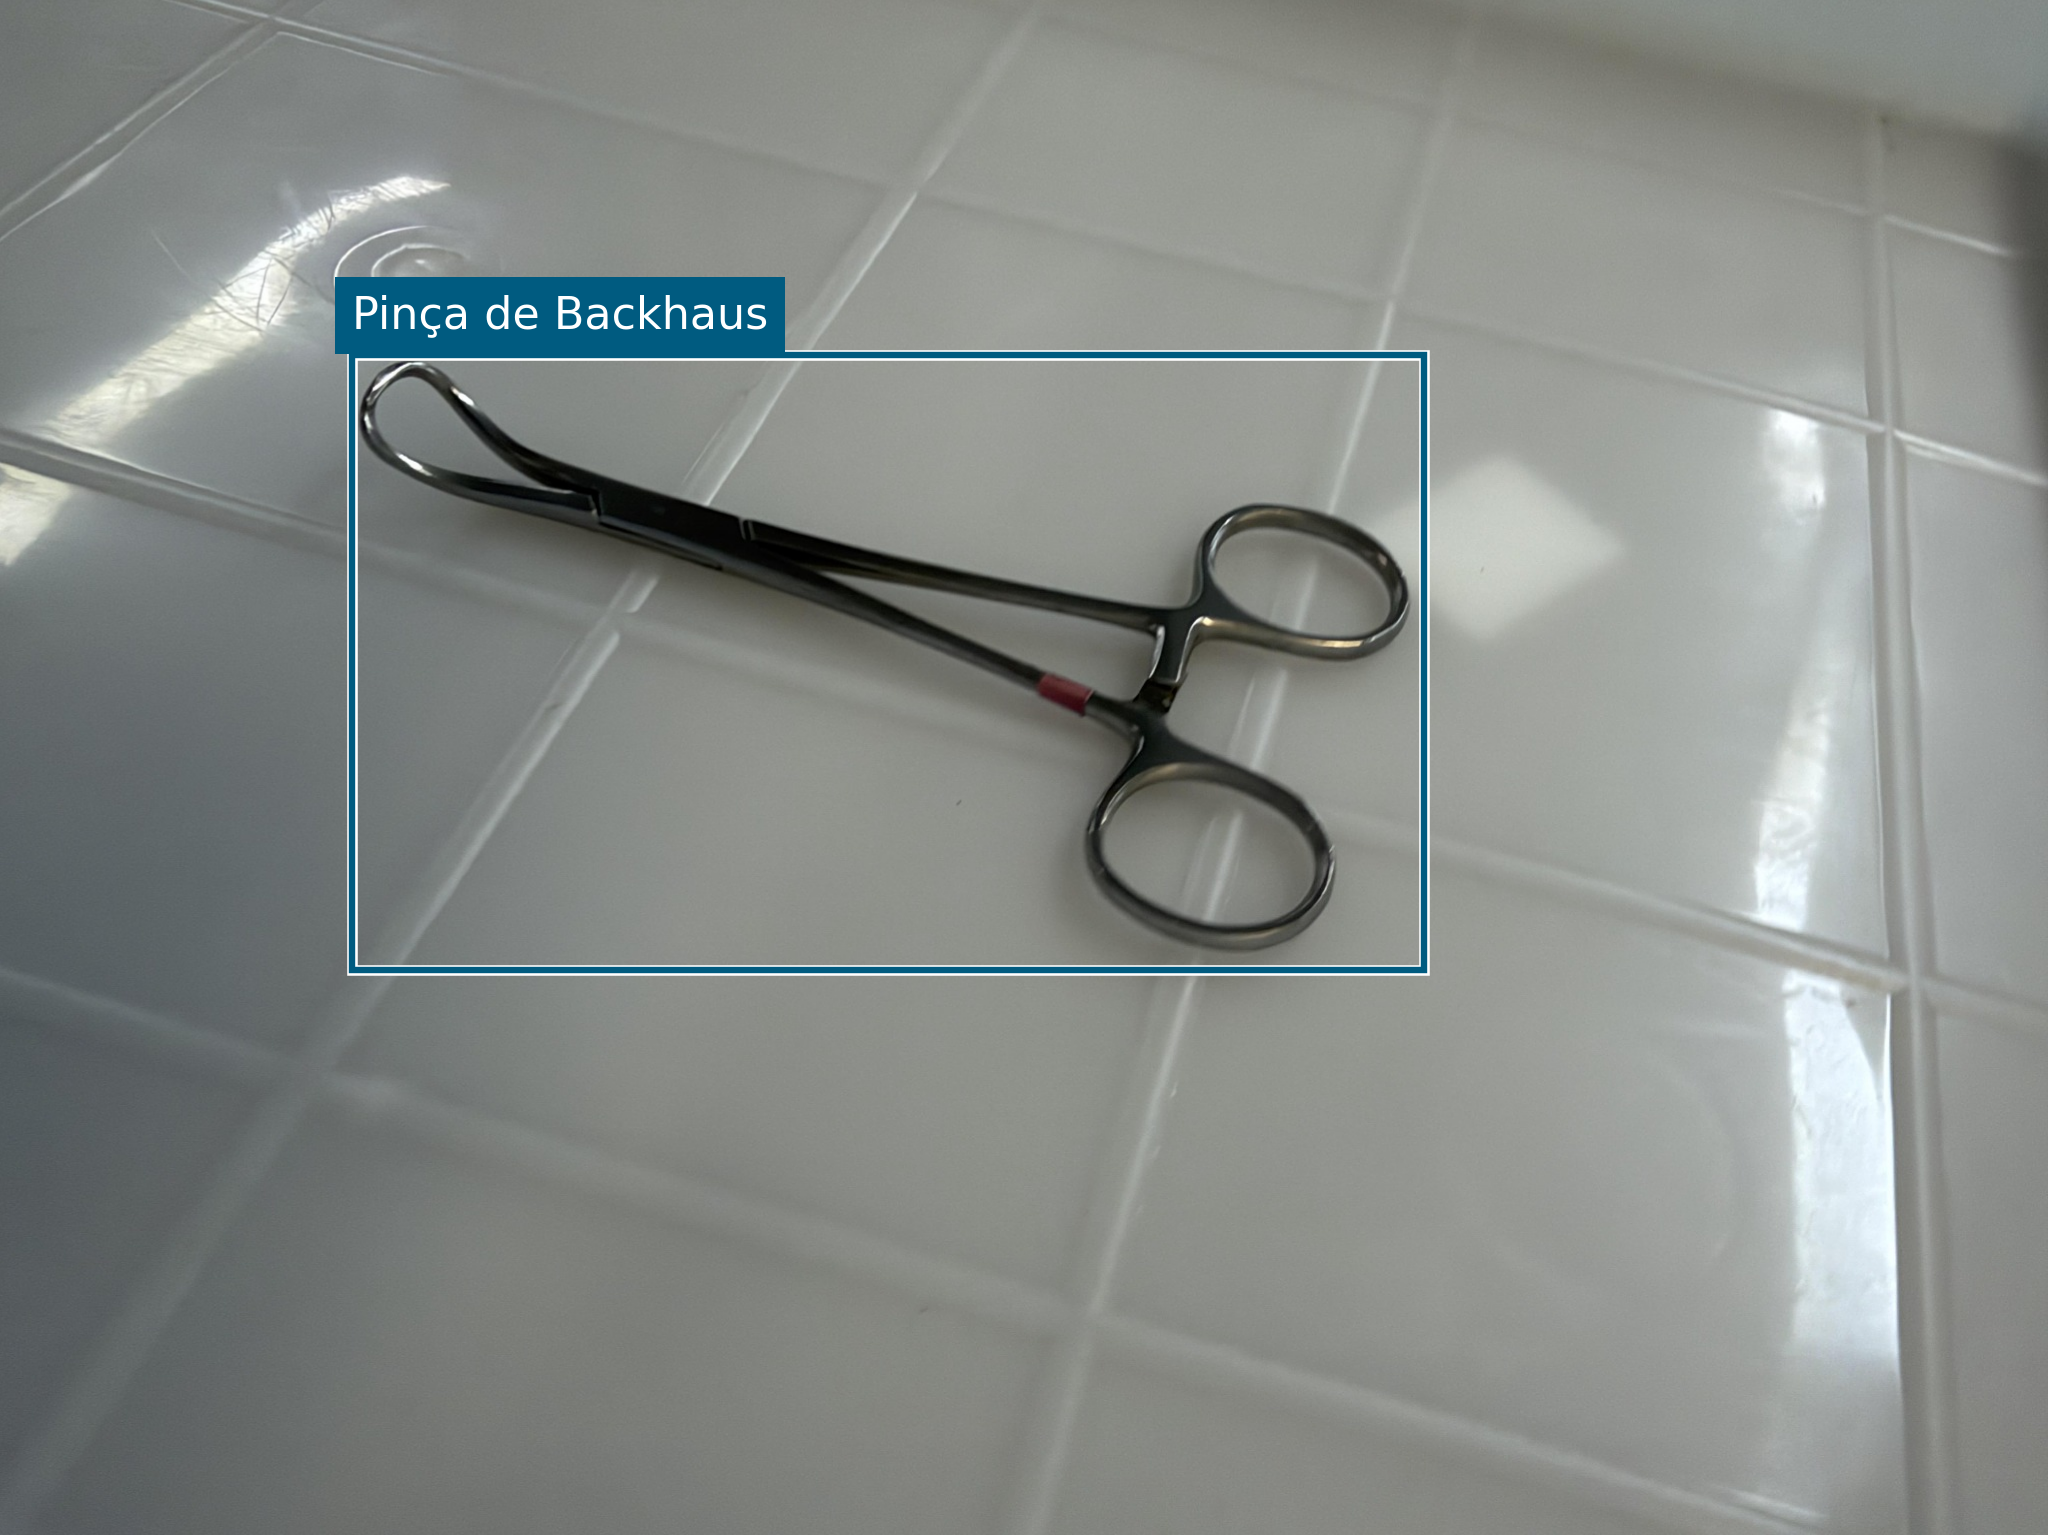
\includegraphics[width=0.72\linewidth,height=0.30\textheight,keepaspectratio]{figuras/exemplo_caixa_delimitadora_hu.png}
\par\smallskip
{\footnotesize Fonte: elaboração própria, a partir de fotografia do conjunto HU-UEL (2026).\par}
\end{figure}
}{}

Para aprender a realizar essa tarefa, o modelo recebe imagens acompanhadas de marcações que indicam a posição e a classe dos objetos. Essas marcações são as anotações de referência: exemplos revisados que orientam o aprendizado e permitem, posteriormente, comparar a resposta do modelo com os objetos efetivamente presentes na imagem. A qualidade desse material importa porque uma caixa mal posicionada, uma classe incorreta ou um instrumento não marcado pode comprometer o aprendizado e a avaliação. Por isso, preparar uma base de imagens envolve selecionar os exemplos, conferir as marcações e organizar nomes e categorias antes do treinamento.

Entre os modelos desenvolvidos para detectar objetos estão o Faster R-CNN e os modelos da família \textit{You Only Look Once} (YOLO). No Faster R-CNN, o processamento inclui a proposta de regiões que podem conter objetos e a análise dessas regiões para classificá-los e ajustar sua localização \parencite{ren2015faster}. A proposta original do YOLO reúne a estimativa das posições e das classes em um processamento da imagem completa, com ênfase na rapidez da detecção \parencite{redmon2016}. Essas abordagens oferecem caminhos distintos para o mesmo problema; a escolha entre elas depende da aplicação, dos dados e dos recursos disponíveis.

Neste estudo, foi selecionada a família YOLO por combinar a localização e a identificação dos objetos em uma solução que permite construir a contagem a partir das detecções. A escolha também encontra apoio em pesquisas sobre instrumentos cirúrgicos, como as de \textcite{ran2023} e \textcite{jiang2023}, que investigaram adaptações de versões anteriores dessa família. Seus resultados motivam a investigação, mas não antecipam o desempenho nas fotografias utilizadas aqui. O modelo adotado é o YOLO26n, variante compacta da família YOLO26. Essa família disponibiliza variantes de diferentes tamanhos, identificadas por n, s, m, l e x, com diferentes necessidades de processamento \parencite{ultralyticsYOLO26intro}. A escolha da variante n considerou os recursos computacionais disponíveis e a possibilidade de avaliar uma solução de menor porte, mantendo a qualidade das detecções e das contagens como questões a serem examinadas experimentalmente.

Essa avaliação exige separar o aprendizado da verificação de seus resultados. As imagens de treinamento são utilizadas para ajustar o modelo; as de validação permitem acompanhar o aprendizado e orientar escolhas de configuração; e as de teste são reservadas para avaliar o desempenho após essas escolhas. Também é necessário preparar as imagens para a entrada da rede. Fotografias de dimensões diferentes são redimensionadas e, quando necessário, recebem preenchimento nas bordas para se adequar ao tamanho de processamento adotado. Esse procedimento facilita a execução computacional, mas pode reduzir detalhes relevantes para distinguir instrumentos semelhantes. As decisões de preparação e avaliação, portanto, fazem parte do problema investigado, e não apenas da execução do programa.

\vspace{\baselineskip}
\phantomsection
\addcontentsline{toc}{subsection}{1.1 Problema de pesquisa e justificativa}
\noindent\textbf{1.1 Problema de pesquisa e justificativa}\par
\vspace{\baselineskip}

A possibilidade de contar instrumentos por imagens é atraente, mas seu uso depende de reconhecer os objetos apesar das variações presentes nas fotografias. Instrumentos metálicos podem produzir reflexos; peças diferentes podem ter formatos semelhantes; e um objeto pode esconder parte de outro. Essas condições dificultam a localização e a identificação, como discutido nos estudos de \textcite{ran2023} e \textcite{jiang2023}. Por isso, a existência de um detector capaz de reconhecer objetos em outras aplicações não é suficiente para concluir que ele atenderá à conferência pretendida no hospital.

A pergunta que orienta esta pesquisa é: em que medida um modelo da família YOLO é tecnicamente viável para identificar e contar instrumentos selecionados da caixa de apendicectomia, nas condições representadas pelas fotografias de avaliação, visando ao apoio à conferência no expurgo e no preparo de caixas cirúrgicas?

Neste contexto, avaliar a viabilidade significa examinar a qualidade das detecções, os erros de contagem, os tempos de treinamento e de processamento das imagens e as situações em que o modelo apresenta dificuldades. Acertar somente o total de objetos não é suficiente. Em uma imagem com dois instrumentos, por exemplo, o modelo pode deixar de reconhecer um deles e marcar indevidamente outra região, produzindo duas detecções apesar do erro. Também pode localizar ambos e trocar suas classes. A análise precisa, portanto, considerar tanto o total quanto a identificação e a localização dos objetos que deram origem à contagem. Os indicadores e os procedimentos utilizados para essa análise são apresentados na metodologia.

A contribuição pretendida é oferecer evidências sobre as possibilidades e os limites dessa abordagem em um conjunto relacionado à rotina do HU-UEL. Para isso, foram reunidas imagens de bases disponíveis na internet e fotografias hospitalares, com revisão dos objetos e de suas anotações. A combinação dessas fontes fornece exemplos para o treinamento, enquanto a avaliação deve mostrar até que ponto o modelo consegue lidar com imagens que não foram utilizadas para ajustá-lo. O estudo trata a contagem automática como um possível recurso de apoio à conferência profissional, sem pressupor que o desempenho em fotografias demonstre, por si só, redução de acidentes ou prontidão para uso assistencial.

\vspace{\baselineskip}
\phantomsection
\addcontentsline{toc}{subsection}{1.2 Objetivos}
\noindent\textbf{1.2 Objetivos}\par
\vspace{\baselineskip}

O objetivo geral é avaliar a viabilidade técnica da detecção e da contagem automática de instrumentos selecionados da caixa de apendicectomia, agrupados em sete categorias gerais, por meio do modelo YOLO26n, visando ao apoio à conferência no expurgo e no preparo de caixas cirúrgicas.

Para alcançar esse objetivo, foram definidos os seguintes objetivos específicos:
\begin{list}{\alph{enumi})}{\usecounter{enumi}\setlength{\leftmargin}{1.25cm}\setlength{\labelsep}{0.5em}\setlength{\itemsep}{0pt}\setlength{\parsep}{0pt}\setlength{\topsep}{0pt}}
\item organizar e revisar as imagens da internet e do HU-UEL, padronizando as categorias e as anotações dos objetos;
\item preparar os conjuntos de treinamento, validação e teste, com controle de duplicatas e agrupamento das imagens relacionadas identificadas;
\item treinar um modelo YOLO para localizar e identificar os instrumentos nas categorias gerais adotadas;
\item avaliar a detecção e a contagem, considerando os resultados totais, os resultados por categoria e a frequência de imagens com contagem correta;
\item analisar os erros e os tempos de treinamento e de processamento por imagem, identificando condições favoráveis e limitações para a aplicação pretendida.
\end{list}

\vspace{\baselineskip}
\phantomsection
\addcontentsline{toc}{subsection}{1.3 Delimitação do estudo}
\noindent\textbf{1.3 Delimitação do estudo}\par
\vspace{\baselineskip}

O experimento utiliza fotografias estáticas e sete categorias gerais: pinças, tesouras, afastadores, porta-agulhas, cabos de bisturi, bicos de aspiração e cúpulas. As cúpulas são recipientes que também integram a contagem dos objetos de interesse. O foco é localizar os objetos e estimar suas quantidades, sem distinguir todos os tipos de instrumentos pertencentes a uma mesma categoria. A correspondência entre os instrumentos selecionados e as categorias utilizadas no treinamento é apresentada na metodologia. Diferenças de tamanho não originam classes distintas.

O agrupamento reúne exemplos de diferentes instrumentos sob um número menor de rótulos e delimita uma tarefa compatível com o objetivo de avaliar a contagem. Essa organização foi considerada pertinente diante da distribuição desigual dos exemplos disponíveis. Entretanto, a pesquisa não compara categorias gerais e específicas e, portanto, não permite afirmar que o agrupamento produziu desempenho superior. Também permanece necessária a análise por categoria, pois reunir instrumentos diferentes não elimina a diversidade visual nem o desequilíbrio da base.

A seleção foi limitada aos objetos de interesse para os quais se obtiveram imagens adequadas. As pinças anatômicas e os cabos de bisturi estão representados somente por imagens da internet na base consolidada. Essas diferenças de cobertura devem ser consideradas ao interpretar os resultados, especialmente quando se discute a aplicação no ambiente hospitalar.

As fotografias incluem instrumentos isolados, alguns conjuntos com vários objetos e bandejas vazias. Embora tenham sido obtidas imagens nos dois ambientes de aplicação pretendidos, o estudo não equivale a uma implantação do sistema no fluxo de trabalho. A avaliação se refere aos objetos visíveis nas fotografias e às condições representadas no conjunto de teste. A conferência integral de uma caixa, o reconhecimento de materiais totalmente encobertos e a demonstração de benefícios durante o uso hospitalar exigem avaliações próprias. Dessa forma, a pesquisa busca estabelecer uma base experimental para decidir como a contagem por visão computacional pode avançar em direção à aplicação pretendida.


\endgroup

% Fundamentação teórica v1. Requer a configuração bibliográfica já instalada.
% Incluir no documento principal; não compilar este arquivo isoladamente.
\begingroup
\justifying
\setlength{\parindent}{1.25cm}
\setlength{\parskip}{0pt}
\setlength{\emergencystretch}{2em}
\onehalfspacing

\phantomsection
\addcontentsline{toc}{section}{2 FUNDAMENTAÇÃO TEÓRICA}
\noindent\textbf{2 FUNDAMENTAÇÃO TEÓRICA}\par
\vspace{\baselineskip}

A contagem de instrumentos por imagem depende de duas etapas logicamente distintas: reconhecer as instâncias visíveis e agregar as detecções aceitas. A primeira envolve localização e classificação; a segunda transforma essas saídas em quantidades. Este capítulo apresenta os conceitos que sustentam essa abordagem, relaciona estudos sobre instrumentos cirúrgicos e discute os cuidados necessários para interpretar os resultados de uma avaliação experimental.

\vspace{\baselineskip}
\phantomsection
\addcontentsline{toc}{subsection}{2.1 Representação visual e aprendizagem supervisionada}
\noindent\textbf{2.1 Representação visual e aprendizagem supervisionada}\par
\vspace{\baselineskip}

Na aprendizagem supervisionada, um modelo é ajustado a partir de exemplos associados a respostas de referência. O objetivo não se limita a reproduzir esses exemplos: espera-se que o modelo apresente desempenho adequado em dados novos. A diferença entre ajuste aos dados disponíveis e generalização é central para interpretar o treinamento de redes neurais \parencite{goodfellow2016}.

Em imagens, as redes convolucionais exploram a organização espacial dos pixels por meio de filtros com parâmetros aprendidos. A aplicação de filtros em diferentes posições permite construir mapas de características, enquanto a composição de camadas possibilita representar padrões progressivamente mais complexos. O compartilhamento de parâmetros reduz a necessidade de aprender uma transformação independente para cada posição da imagem \parencite{goodfellow2016}. Isso não elimina, entretanto, a influência das condições de aquisição sobre a resposta da rede.

Para instrumentos cirúrgicos, detalhes como a extremidade ativa, a presença de dentes e a curvatura podem ser decisivos para distinguir classes específicas. Uma fotografia em alta resolução pode conter esses detalhes, mas o redimensionamento para a entrada do detector pode torná-los pouco visíveis. Por outro lado, uma imagem que mostra apenas a ponta pode favorecer a identificação de uma característica e oferecer pouca informação sobre a localização do instrumento completo. Essas situações representam exigências diferentes para o sistema e precisam ser consideradas na seleção dos exemplos de treinamento e avaliação.

Classificação de imagens, detecção de objetos e segmentação de instâncias também produzem respostas diferentes. A classificação associa categorias à imagem; a detecção localiza objetos por caixas e atribui classes; a segmentação de instâncias delimita regiões de pixels de cada objeto. Na formulação original do YOLO, a rede estima caixas delimitadoras e probabilidades de classe a partir da imagem completa \parencite{redmon2016}. Para a contagem aqui investigada, a unidade de interesse é a instância de instrumento, e uma caixa deve representar um objeto, mesmo que ele tenha partes separadas visualmente por oclusão.

Uma caixa delimitadora alinhada aos eixos descreve uma região retangular, não o contorno exato do instrumento. Por isso, pode incluir fundo e partes de outros objetos, sobretudo quando o instrumento está inclinado ou sobreposto. Converter um polígono em sua caixa envolvente permite utilizar a anotação em detecção, mas descarta a informação fina de contorno. A conversão também não corrige automaticamente um polígono que abranja componentes fora do objeto desejado; essa adequação depende de revisão da anotação.

\vspace{\baselineskip}
\phantomsection
\addcontentsline{toc}{subsection}{2.2 Detecção com a família YOLO}
\noindent\textbf{2.2 Detecção com a família YOLO}\par
\vspace{\baselineskip}

\textcite{redmon2016} propuseram tratar a detecção como uma predição conjunta de localização e classe em uma única rede. Essa formulação utiliza informação da imagem completa para estimar os objetos presentes. A designação YOLO, contudo, passou a reunir modelos com mudanças de arquitetura e treinamento; características da proposta original não devem ser atribuídas automaticamente às versões posteriores.

O YOLO26 é descrito por \textcite{jocher2026} como uma família com diferentes escalas de modelo e suporte a tarefas de visão computacional. Para detecção, os autores apresentam uma arquitetura com duas cabeças e a possibilidade de inferência sem uma etapa separada de supressão de não máximos, conhecida pela sigla NMS. Essa supressão é utilizada em detectores para reduzir caixas redundantes a partir de suas pontuações e sobreposição. A existência de um caminho de inferência sem NMS não dispensa a conferência da configuração efetivamente utilizada pelo software.

O estudo de \textcite{jocher2026} está disponível como \textit{preprint}; sua descrição técnica é útil para identificar o modelo, mas não constitui validação independente para a aplicação hospitalar deste trabalho. Resultados obtidos pelos autores em bases de referência e dispositivos específicos não antecipam a precisão nem o tempo de execução nas imagens de instrumentos e no equipamento aqui empregado.

O uso de pesos pré-treinados permite iniciar o ajuste de um detector a partir de parâmetros já aprendidos, em vez de partir apenas de uma inicialização aleatória. Ainda assim, o novo treinamento precisa adaptar a saída às classes e aos exemplos disponíveis. O reaproveitamento de representações entre tarefas integra as estratégias de transferência de aprendizagem discutidas por \textcite{goodfellow2016}. No presente problema, uma categoria reconhecida em uma base genérica não equivale à distinção entre instrumentos visualmente próximos.

A escolha entre variantes de menor e maior capacidade envolve recursos computacionais, tempo disponível e desempenho observado. Um modelo maior pode exigir mais memória e processamento sem resolver problemas de anotação, baixa diversidade ou ausência de exemplos representativos. Consequentemente, a comparação de variantes precisa manter condições de avaliação compatíveis e apresentar os resultados medidos, sem tomar o tamanho do modelo como evidência antecipada de superioridade.

\vspace{\baselineskip}
\phantomsection
\addcontentsline{toc}{subsection}{2.3 Estudos sobre reconhecimento de instrumentos cirúrgicos}
\noindent\textbf{2.3 Estudos sobre reconhecimento de instrumentos cirúrgicos}\par
\vspace{\baselineskip}

\textcite{ran2023} investigaram uma adaptação do YOLOv7x para detectar instrumentos cirúrgicos. O trabalho aborda dificuldades relacionadas à semelhança entre objetos, à disposição dos instrumentos e às condições visuais das imagens. Sua contribuição sustenta o uso da detecção como abordagem pertinente ao problema, mas os resultados relatados estão vinculados às classes, às imagens e ao protocolo empregados naquele estudo.

\textcite{jiang2023} estudaram uma versão modificada do YOLOv5 para reconhecimento de instrumentos. A base descrita pelos autores inclui imagens com instrumentos sem empilhamento e com empilhamento, utilizando tecido azul como fundo. A consideração de sobreposição aproxima o estudo de uma dificuldade relevante para a contagem, pois a presença de vários objetos exige que o detector separe instâncias e mantenha sua identificação mesmo quando parte delas está encoberta.

Os dois trabalhos fornecem referências de aplicação, mas não estabelecem uma comparação direta com este TCC. Diferenças na composição das bases, no número de classes, nas condições de captura e nos critérios de avaliação impedem interpretar métricas publicadas como metas automaticamente transferíveis. Tampouco a adoção de uma versão mais recente da família YOLO garante superar os resultados de versões anteriores avaliadas em outros dados.

A contribuição deste trabalho concentra-se na avaliação da contagem para o conjunto de instrumentos selecionado e nas condições documentadas de aquisição e organização das imagens. Isso exige observar não apenas se há detecções, mas quais instrumentos foram omitidos, confundidos ou contados mais de uma vez. As orientações de cirurgia segura da Organização Mundial da Saúde contextualizam a importância da conferência de materiais \parencite{oms2009}; contudo, uma avaliação computacional em fotografias não demonstra, por si só, redução de eventos adversos ou substituição de procedimentos assistenciais.

\vspace{\baselineskip}
\phantomsection
\addcontentsline{toc}{subsection}{2.4 Qualidade dos dados e independência da avaliação}
\noindent\textbf{2.4 Qualidade dos dados e independência da avaliação}\par
\vspace{\baselineskip}

A separação entre treinamento, validação e teste atribui funções diferentes aos dados. O treinamento ajusta os parâmetros; a validação auxilia a escolha de configurações; o teste estima o desempenho após essas escolhas. Utilizar repetidamente o teste para orientar modificações compromete sua função de avaliação independente. \textcite{kapoor2023} discutem como o vazamento de informação pode levar a conclusões excessivamente otimistas em pesquisas baseadas em aprendizagem de máquina.

No caso de fotografias de instrumentos, a independência não pode ser verificada apenas pelo nome do arquivo. Cópias recomprimidas, recortes e transformações de uma mesma fotografia podem preservar grande parte do conteúdo visual. Imagens capturadas em sequência também podem compartilhar objeto, posição, iluminação e fundo. Se exemplos fortemente relacionados forem distribuídos entre treinamento e teste, a avaliação pode refletir a familiaridade com aquela aquisição, em vez da resposta a uma condição nova. O controle desse risco demanda rastreabilidade e agrupamento dos exemplos relacionados antes da divisão.

Identidade digital e similaridade visual são evidências diferentes. Um resumo criptográfico permite comparar os bytes dos arquivos, mas uma alteração de compressão pode modificar esses bytes sem produzir uma mudança visual relevante. Métodos perceptuais auxiliam a busca por candidatos semelhantes, porém não substituem a análise dos casos ambíguos: instrumentos distintos podem ter aparência próxima. O procedimento adotado precisa registrar os critérios e as decisões, sem afirmar que um único limiar garante ausência de vazamento.

O aumento de dados produz variações dos exemplos de treinamento, como mudanças de orientação e aparência. Essas transformações são formas de introduzir variação e regularizar o aprendizado \parencite{goodfellow2016}. Elas não criam novas sessões independentes de coleta. Quando aplicadas durante o carregamento dos lotes, também não correspondem necessariamente a uma nova quantidade fixa de arquivos no disco. Por essa razão, é mais informativo registrar as técnicas, suas probabilidades e as épocas de aplicação do que apresentar uma multiplicação arbitrária do número de imagens.

Outro aspecto é a distribuição conjunta de classes e origens. Uma classe numerosa pode estar representada quase exclusivamente por imagens da internet, enquanto outra pode ter maior variedade de fotografias hospitalares. Assim, a quantidade de exemplos, isoladamente, não expressa a cobertura das condições de uso. Para este estudo, resultados separados por origem e por classe ajudam a localizar limitações que uma média global pode ocultar. Classes sem exemplos hospitalares de teste não permitem estimar diretamente seu desempenho nesse domínio.

\vspace{\baselineskip}
\phantomsection
\addcontentsline{toc}{subsection}{2.5 Avaliação da detecção}
\noindent\textbf{2.5 Avaliação da detecção}\par
\vspace{\baselineskip}

A avaliação exige comparar predições com anotações de referência segundo critérios explícitos. A interseção sobre união, ou IoU, mede a sobreposição entre a caixa predita $B_p$ e a caixa de referência $B_r$:
\begin{equation}
\mathrm{IoU}(B_p,B_r)=\frac{|B_p\cap B_r|}{|B_p\cup B_r|}.
\label{eq:fund_iou}
\end{equation}
Na Equação~\ref{eq:fund_iou}, as barras representam áreas. A correspondência de uma detecção depende da classe, do limiar de IoU e da regra de associação entre predições e referências. Na avaliação usual de instâncias individuais, uma referência não deve contabilizar várias predições como acertos \parencite{padilla2021}.

Sejam $VP$, $FP$ e $FN$ as quantidades de verdadeiros positivos, falsos positivos e falsos negativos. Precisão e revocação são expressas, para denominadores não nulos, por
\begin{equation}
P=\frac{VP}{VP+FP},\qquad R=\frac{VP}{VP+FN}.
\label{eq:fund_pr}
\end{equation}
A precisão relaciona os acertos às detecções aceitas; a revocação relaciona os acertos aos objetos de referência. A precisão média, AP, resume a curva precisão--revocação segundo uma regra de integração ou interpolação. A mAP agrega AP entre classes. As convenções de cálculo precisam ser informadas, pois diferenças de implementação afetam a comparação \parencite{padilla2021}.

Na notação usual, mAP@0,50 utiliza IoU de 0,50; mAP@0,50:0,95 agrega os limiares de 0,50 a 0,95 em passos de 0,05. Esses valores não representam a porcentagem de fotografias cuja contagem está correta. Além disso, o limiar de IoU empregado para julgar a localização não é o limiar de confiança utilizado para aceitar uma predição. A metodologia deve registrar ambos e distinguir a avaliação da curva de detecção da configuração usada para produzir as contagens.

Uma caixa imprecisa pode ainda contribuir com uma unidade para a contagem, enquanto uma classificação errada pode preservar o total e alterar a composição por instrumento. Por isso, as métricas de detecção e de contagem respondem a perguntas complementares. A análise dos erros deve relacionar o resultado numérico às caixas e às classes preditas.

\vspace{\baselineskip}
\phantomsection
\addcontentsline{toc}{subsection}{2.6 Contagem por detecção e critérios de interpretação}
\noindent\textbf{2.6 Contagem por detecção e critérios de interpretação}\par
\vspace{\baselineskip}

Considere $N$ imagens e $C$ classes. Para a imagem $i$, seja $D_i$ o conjunto de detecções aceitas após a aplicação dos critérios de confiança e pós-processamento definidos. A contagem estimada da classe $c$ pode ser escrita como
\begin{equation}
\widehat{n}_{ic}=\sum_{d\in D_i}\mathbf{1}[\operatorname{classe}(d)=c],
\qquad \widehat{n}_i=\sum_{c=1}^{C}\widehat{n}_{ic},
\label{eq:fund_contagem}
\end{equation}
em que $\mathbf{1}[\cdot]$ vale um quando a condição é verdadeira e zero caso contrário. Os índices matemáticos das classes vão de um a $C$, independentemente da numeração adotada nos arquivos de anotação. Essa formulação explicita que a contagem depende das detecções efetivamente aceitas, não de todas as hipóteses internas da rede.

Se $n_i$ é a contagem total de referência, o erro absoluto médio total é
\begin{equation}
\mathrm{MAE}_{\mathrm{total}}=\frac{1}{N}\sum_{i=1}^{N}|\widehat{n}_i-n_i|.
\label{eq:fund_mae}
\end{equation}
O valor informa quantos objetos, em média por imagem, separam a estimativa do total anotado. Para examinar a identificação, calcula-se também o erro por classe, substituindo os totais por $\widehat{n}_{ic}$ e $n_{ic}$. Quando a maioria das imagens não contém determinada classe, a média calculada sobre todas as imagens pode ser pequena mesmo com falhas nos exemplos positivos; convém, portanto, explicitar o suporte e separar a análise de presença e ausência.

A proporção de imagens com total exato e a proporção com todas as contagens por classe corretas podem ser definidas, respectivamente, por
\begin{equation}
E_{\mathrm{total}}=\frac{1}{N}\sum_{i=1}^{N}\mathbf{1}[\widehat{n}_i=n_i],
\label{eq:fund_exato_total}
\end{equation}
\begin{equation}
E_{\mathrm{classes}}=\frac{1}{N}\sum_{i=1}^{N}
\mathbf{1}[\widehat{n}_{ic}=n_{ic}\ \mathrm{para\ todo}\ c].
\label{eq:fund_exato_classes}
\end{equation}
Essas expressões são definições operacionais para organizar a avaliação deste problema, e não resultados experimentais. Uma omissão e uma detecção indevida podem se compensar no total; até a igualdade das contagens por classe pode coexistir com erros de localização. Nenhum desses indicadores substitui a inspeção das detecções.

O Quadro~\ref{qua:fund_interpretacao} sintetiza as diferenças entre as perguntas de avaliação. O agrupamento em categorias gerais exige atenção adicional: confundir duas classes específicas pertencentes ao mesmo grupo deixa de ser um erro de classe nessa representação. Logo, um resultado superior com categorias gerais não demonstra, por si só, melhor reconhecimento específico.

\begin{table}[htbp]
\centering
\begin{minipage}{\linewidth}
\singlespacing
\refstepcounter{table}\label{qua:fund_interpretacao}
\noindent Quadro \thetable{} -- Interpretação complementar dos resultados\par
\smallskip
\small
\setlength{\tabcolsep}{5pt}
\renewcommand{\arraystretch}{1.25}
\begin{tabular}{|p{0.24\linewidth}|p{0.32\linewidth}|p{0.32\linewidth}|}
\hline
\textbf{Aspecto} & \textbf{Pergunta respondida} & \textbf{Limite de interpretação}\\\hline
Detecção & Os instrumentos foram localizados e classificados? & Não informa diretamente a frequência de contagens exatas.\\\hline
Contagem total & Quantos objetos há na imagem? & Erros podem se compensar; classes podem estar trocadas.\\\hline
Contagem por classe & A composição por instrumento está correta? & Contagens iguais não garantem caixas corretas.\\\hline
Imagens sem objetos & O sistema produz detecções indevidas? & Bandejas vazias não representam todos os fundos possíveis.\\\hline
Tempo de execução & Qual o custo no equipamento utilizado? & Depende da resolução e das etapas incluídas na medição.\\\hline
\end{tabular}
\par\smallskip
\footnotesize Fonte: elaboração própria.
\end{minipage}
\end{table}

Finalmente, a viabilidade técnica depende do cenário avaliado. Fotografias de objetos isolados, imagens com poucos instrumentos e fotografias de bandejas completas impõem dificuldades distintas. Uma conclusão favorável em um desses cenários deve permanecer limitada às condições observadas. Neste trabalho, a articulação entre detecção, contagem, análise visual dos erros e custo computacional fornece a base para essa delimitação, sem converter desempenho experimental em comprovação de segurança clínica.

\endgroup

% !TeX root = 0_TCC.tex
% Metodologia v2 — 01/11/2026. Não compilar isoladamente.
% Mantém o padrão do template e a bibliografia já instalada.
\begingroup
\justifying
\setlength{\parindent}{1.25cm}
\setlength{\parskip}{0pt}
\setlength{\emergencystretch}{2em}
\onehalfspacing
\renewcommand{\tablename}{Tabela}
\captionsetup[table]{labelsep=endash,justification=raggedright,singlelinecheck=false,font=small}

\phantomsection
\addcontentsline{toc}{section}{3 METODOLOGIA}
\noindent\textbf{3 METODOLOGIA}\par
\nobreak\vspace{\baselineskip}\nobreak

Esta pesquisa avalia se um modelo de visão computacional consegue localizar instrumentos cirúrgicos em fotografias e contar quantos exemplares de cada categoria estão presentes. Para isso, foi organizado um experimento com imagens da internet e do Hospital Universitário da Universidade Estadual de Londrina (HU-UEL). Cada fotografia constitui uma entrada para o modelo; cada instrumento marcado nessa fotografia constitui um objeto de referência. Essa distinção permite avaliar separadamente o reconhecimento dos instrumentos e o acerto das quantidades.

O procedimento foi organizado em cinco etapas: seleção das fontes; limpeza e anotação das imagens; reunião e separação dos dados; treinamento do modelo; e avaliação da detecção e da contagem. A sequência parte da preparação dos exemplos que o modelo utilizará para aprender e termina na análise de fotografias reservadas para o teste. Assim, o desempenho será examinado em dados que não participam do ajuste dos pesos da rede.

Os instrumentos selecionados têm como referência a caixa de apendicectomia, isto é, o conjunto de materiais utilizado na cirurgia de retirada do apêndice. A aplicação pretendida abrange a conferência de instrumentos no expurgo e no preparo, ambientes que integram o fluxo de processamento de materiais descrito por \textcite{moreto2025}. O experimento avalia a contagem em fotografias, sem abranger esterilidade, integridade física ou funcionamento dos instrumentos. Portanto, a viabilidade investigada é a de um apoio computacional à conferência, dentro das condições representadas pela base de imagens.

\vspace{\baselineskip}
\phantomsection
\addcontentsline{toc}{subsection}{3.1 Constituição e procedência da base de imagens}
\noindent\textbf{3.1 Constituição e procedência da base de imagens}\par
\nobreak\vspace{\baselineskip}\nobreak

A base de imagens reuniu duas origens complementares. Os conjuntos públicos ofereceram exemplos previamente anotados de diferentes instrumentos, enquanto as fotografias do HU-UEL acrescentaram registros dos materiais nos ambientes em que se pretende utilizar a contagem. As fontes da internet receberam os identificadores DS01 a DS07 para permitir acompanhar sua contribuição durante a organização. Esses identificadores são utilizados nas tabelas deste capítulo.

Os conjuntos DS01, DS03, DS04 e DS05 foram obtidos no Roboflow; o DS06, no Kaggle; e o DS07, no Hugging Face. Os endereços das fontes são indicados em nota.\footnote{DS01: \url{https://universe.roboflow.com/fmsurg/isef-training-dataset-p360u/dataset/1}; DS03: \url{https://universe.roboflow.com/surgical-tools-hnzri/surgical_tools-6b7ze}; DS04: \url{https://universe.roboflow.com/new-workspace-fjl7e/set_1_11/dataset/2}; DS05: \url{https://universe.roboflow.com/practicum-ii-iii/suturing-kit-tools}; DS06: \url{https://www.kaggle.com/datasets/dilavado/labeled-surgical-tools}; DS07: \url{https://huggingface.co/datasets/joonhaim/surgical-tool-recognition-full-multiview}.} O DS02 foi descartado integralmente após a revisão identificar imagens já presentes no DS01, inclusive versões com alterações de borda e ampliação. Dessa forma, seis conjuntos externos contribuíram para a base final.

As fotografias do HU-UEL foram organizadas inicialmente por instrumento e, em casos específicos, por composição de objetos. Entre as composições anotadas estão imagens com pinça dente de rato, pinça Backhaus e cúpula, além de imagens contendo uma tesoura Metzenbaum reta e outra curva. Também foram incorporadas 100 fotografias de bandejas vazias como exemplos negativos. Imagens sem instrumentos possuem arquivo de anotação vazio; por isso, a ausência de objetos nesses casos é intencional e não deve ser interpretada como falha de rotulagem.

As fotografias do HU-UEL foram produzidas por uma enfermeira em diferentes dias, ao longo de aproximadamente três semanas, nos ambientes de expurgo e preparo. Foi utilizado um \textbf{iPhone xx}. No primeiro dia, parte das imagens foi registrada em HEIC; posteriormente, o aparelho foi configurado no modo de alta compatibilidade, passando a produzir arquivos JPEG. As primeiras imagens foram aproveitadas após conversão para um formato compatível com o fluxo de anotação. Os registros utilizados mostram instrumentos e superfícies de apoio, sem pessoas ou procedimentos cirúrgicos em andamento.

A produção em dias e ambientes distintos acrescenta variação às fotografias, mas não permite assumir que todos os registros sejam independentes: imagens próximas podem mostrar o mesmo instrumento, sobre a mesma superfície, com pequenas mudanças de posição. Essa característica foi considerada na busca de repetições e na separação dos dados, descritas na Seção 3.3.

A Tabela~\ref{tab:met-origens} apresenta a composição após a seleção e a revisão. Essas quantidades descrevem os dados utilizados no experimento, e não resultados de desempenho do modelo. A contagem foi realizada por scripts Python que verificaram os pares de imagens e anotações. Uma fotografia com três instrumentos acrescenta uma unidade ao total de imagens e três ao total de objetos; uma bandeja vazia acrescenta apenas uma imagem.

\begin{table}[htbp]
\centering
\begin{minipage}{0.92\linewidth}
\singlespacing\small
\caption{Composição da base consolidada por origem}
\label{tab:met-origens}
\centering
\begin{tabular}{lrr}
\hline
Origem & Imagens & Objetos anotados \\
\hline
DS01 & 289 & 414 \\
DS03 & 115 & 129 \\
DS04 & 249 & 382 \\
DS05 & 85 & 85 \\
DS06 & 2.964 & 4.149 \\
DS07 & 1.008 & 1.008 \\
Subtotal da internet & 4.710 & 6.167 \\
HU-UEL & 5.617 & 6.547 \\
\hline
Total & 10.327 & 12.714 \\
\hline
\end{tabular}\par
\vspace{0.35em}\raggedright
Fonte: elaboração própria, a partir da revisão e contagem dos dados por scripts Python (2026).\par
Nota: as 100 imagens negativas estão incluídas no total do HU-UEL e não acrescentam objetos.
\end{minipage}
\end{table}

\vspace{\baselineskip}
\phantomsection
\addcontentsline{toc}{subsection}{3.2 Seleção, anotação e padronização dos instrumentos}
\noindent\textbf{3.2 Seleção, anotação e padronização dos instrumentos}\par
\nobreak\vspace{\baselineskip}\nobreak

Antes do treinamento, as imagens e suas anotações passaram por limpeza e conferência. Essa preparação é necessária porque o modelo aprende a partir dos exemplos disponíveis: uma classe incorreta ensina uma associação inadequada, um instrumento sem caixa pode ser interpretado como fundo e uma repetição entre treino e teste pode tornar a avaliação excessivamente favorável. A revisão procurou reduzir esses problemas antes de reunir os conjuntos.

Foram retiradas imagens de baixa qualidade que impediam identificar o instrumento, materiais incompatíveis com a caixa selecionada e versões repetidas reconhecidas durante a inspeção. Entre as repetições estavam imagens com espelhamento, alterações de perspectiva ou regiões cobertas por quadrados escuros, provenientes de aumento de dados aplicado previamente. Sempre que possível, foi preservada a versão original de melhor qualidade. A seleção considerou o conteúdo da fotografia, e não apenas seu nome ou o nome da classe no conjunto de origem. Dúvidas sobre instrumentos específicos foram esclarecidas com a enfermeira colaboradora.

Instrumentos visualmente semelhantes, mas fora do escopo, não foram incluídos apenas para aumentar o volume da base. Quando sua presença poderia gerar supervisão contraditória, optou-se pela retirada da imagem, inclusive se ela também apresentasse um objeto desejado. Um exemplo foi o afastador Army-Navy, cuja aparência em determinadas posições se aproxima daquela do Farabeuf. Essa escolha delimita o domínio do experimento: o detector não é avaliado como classificador universal de instrumentos semelhantes aos selecionados.

A revisão dos conjuntos externos foi realizada com apoio do CVAT e de inspeções no Roboflow. As fotografias do HU-UEL foram anotadas no X-AnyLabeling. Anotar uma imagem, neste estudo, significa traçar um retângulo que envolva cada instrumento e atribuir a ele uma classe. Esses retângulos, ou caixas delimitadoras, constituem as referências utilizadas para ensinar e avaliar o detector. Foram utilizadas caixas horizontais, com lados paralelos às bordas da fotografia, mesmo quando o instrumento estava inclinado.

As anotações foram exportadas no formato YOLO para detecção. Cada linha do arquivo TXT representa um objeto e contém o identificador da classe, as coordenadas do centro da caixa, sua largura e sua altura. As quatro medidas são divididas pelas dimensões da imagem, ficando normalizadas entre zero e um. Por exemplo, uma largura de 0,25 representa um quarto da largura da fotografia. A imagem e seu TXT compartilham o mesmo nome-base, permitindo associá-los sem depender da ordem dos arquivos na pasta.

Nos conjuntos com polígonos, a conversão para detecção utilizou os menores e maiores valores de cada coordenada para obter a caixa envolvente de cada instância. Esse procedimento conserva a extensão espacial do contorno anotado, mas não verifica sua pertinência semântica. Por isso, caixas que abrangiam componentes indesejados, como tubos conectados ao bico de aspiração ou partes além do cabo de bisturi, foram submetidas à revisão manual. No DS07, as anotações convertidas de JSONL foram inspecionadas visualmente, e foram mantidas as classes correspondentes a porta-agulhas e cabos de bisturi.

Para utilizar os mesmos dados em diferentes níveis de detalhe, foram preservadas duas organizações das classes, também chamadas de taxonomias. A específica distingue 17 instrumentos ou variantes, incluindo Kelly, Mayo e Metzenbaum retas e curvas. A geral reúne essas classes em sete categorias e foi utilizada no treinamento principal. A correspondência é fixa: cada objeto de uma classe específica recebe uma única categoria geral. O agrupamento reduz o número de nomes que o modelo precisa distinguir, mas conserva diferenças visuais dentro de categorias como pinças; não se pressupõe que todos os instrumentos agrupados tenham a mesma aparência.

Diferenças de tamanho não originam classes distintas. Porta-agulhas, cúpula e bico de aspiração foram mantidos em categorias próprias. A pinça Collin coração não integra esta etapa por falta de imagens, e a Kocher curva não pertence ao conjunto selecionado. Os exemplares Yankauer aceitos na conferência foram reunidos à categoria de bicos de aspiração.

A Tabela~\ref{tab:met-taxonomias} explicita a correspondência entre as taxonomias e a quantidade de objetos em cada categoria geral. Os nomes em português são utilizados na apresentação do trabalho; os identificadores em inglês são empregados nos arquivos de treinamento. As duas organizações mantêm as mesmas caixas e divisões, alterando apenas os identificadores de classe. Portanto, não constituem duas bases independentes.

\begin{table}[htbp]
\centering
\begin{minipage}{\linewidth}
\singlespacing\small
\caption{Correspondência entre classes específicas e categorias gerais}
\label{tab:met-taxonomias}
\begin{tabular}{p{0.19\linewidth}p{0.61\linewidth}r}
\hline
Categoria geral & Classes específicas representadas & Objetos \\
\hline
Pinças & Allis; anatômica; Backhaus; Kelly curva; Kelly reta; Foerster; dente de rato; Kocher reta & 4.907 \\
Tesouras & Mayo curva; Mayo reta; Metzenbaum curva; Metzenbaum reta & 3.976 \\
Afastadores & Farabeuf & 848 \\
Porta-agulhas & Porta-agulhas & 760 \\
Cabos de bisturi & Cabo de bisturi & 1.673 \\
Bicos de aspiração & Bico de aspiração, incluindo exemplares Yankauer aceitos na revisão & 244 \\
Cúpulas & Cúpula & 306 \\
\hline
Total & 17 classes específicas e 7 categorias gerais & 12.714 \\
\hline
\end{tabular}\par
\vspace{0.35em}\raggedright
Fonte: elaboração própria, a partir da revisão e contagem dos dados por scripts Python (2026).
\end{minipage}
\end{table}

A representação é desigual entre classes e origens. Por exemplo, as pinças anatômicas e os cabos de bisturi da base consolidada provêm exclusivamente da internet. Consequentemente, um resultado agregado satisfatório não demonstra desempenho hospitalar para todas as classes. Essa diferença deve ser considerada na análise dos erros e na apresentação dos resultados por origem.

\vspace{\baselineskip}
\phantomsection
\addcontentsline{toc}{subsection}{3.3 Consolidação, verificação e separação dos dados}
\noindent\textbf{3.3 Consolidação, verificação e separação dos dados}\par
\nobreak\vspace{\baselineskip}\nobreak

Neste estudo, consolidação significa reunir os conjuntos selecionados em uma única base organizada, compatibilizando nomes de classes, formatos de anotação e estrutura de pastas. Esse processo foi executado por scripts Python sobre cópias dos arquivos, preservando os conjuntos originais. Cada imagem consolidada manteve uma identificação de sua origem, de suas classes e da divisão à qual foi destinada. A preparação ocorreu no Windows, e a base organizada foi transferida para o Mac utilizado no treinamento.

A conferência automática verificou se cada imagem podia ser aberta, se possuía a anotação correspondente e se os identificadores de classe estavam previstos no mapeamento. Também foram examinadas as coordenadas das caixas, incluindo dimensões positivas e limites válidos. Os arquivos vazios foram tratados separadamente para distinguir as bandejas sem instrumentos de uma possível ausência de anotação. As duas taxonomias foram comparadas para verificar a manutenção das mesmas imagens, caixas e divisões, com alteração apenas das classes.

A busca por repetições combinou comparação de arquivos, comparação dos pixels decodificados e semelhança visual. Para isso, foram utilizados resumos digitais, chamados \textit{hashes}: o SHA-256 permitiu conferir a integridade dos arquivos comparados, enquanto o dHash forneceu uma assinatura simplificada da aparência. Assinaturas perceptuais próximas indicaram candidatos à revisão, mas não foram tratadas como prova suficiente de duplicação. Fotografias de instrumentos diferentes sobre o mesmo fundo podem apresentar grande semelhança nessa representação.

Os candidatos foram examinados visualmente para distinguir cópias de fotografias diferentes. Quando uma mesma imagem apareceu em resoluções distintas, a versão de melhor qualidade foi priorizada. Fotografias relacionadas por repetição ou sequência identificada foram reunidas em grupos destinados à mesma divisão. Dessa forma, procurou-se evitar que uma versão fosse utilizada no aprendizado e outra muito próxima fosse usada para avaliar o mesmo modelo.



O agrupamento procura reduzir a dependência entre dados usados para aprender e dados usados para avaliar. Como discutem \textcite{kapoor2023}, falhas na separação podem produzir conclusões excessivamente otimistas. Entretanto, a ausência de grupos cadastrados em mais de uma divisão não comprova independência de todas as sessões de aquisição. A base contém imagens de instrumentos reposicionados em cenários semelhantes, e os registros disponíveis não permitem reconstruir integralmente todas as sessões das fontes externas. Essa restrição permanece como limitação do experimento.

Após a organização, a base foi separada em treino, validação e teste. O treino fornece os exemplos utilizados para ajustar os pesos da rede. A validação acompanha o aprendizado e permite selecionar o estado do modelo e o limiar de confiança. O teste permanece reservado para avaliar o procedimento após essas escolhas. A distribuição final se aproxima de 80\%, 10\% e 10\%, respectivamente, com pequenos ajustes necessários para manter os grupos identificados na mesma divisão.

A Tabela~\ref{tab:met-splits} apresenta as quantidades efetivas. A mesma divisão foi preservada nas duas taxonomias, permitindo uma eventual comparação sobre as mesmas fotografias. Entre os exemplos negativos, 80 bandejas vazias pertencem ao treino, dez à validação e dez ao teste. A separação por grupos reduz um risco de dependência, mas não equivale a uma divisão completa por dia, paciente ou hospital: as fontes disponíveis não fornecem todos esses metadados.

\begin{table}[htbp]
\centering
\begin{minipage}{0.92\linewidth}
\singlespacing\small
\caption{Distribuição das imagens e dos objetos por divisão}
\label{tab:met-splits}
\centering
\begin{tabular}{lrr}
\hline
Divisão & Imagens & Objetos anotados \\
\hline
Treino & 8.304 & 10.044 \\
Validação & 1.015 & 1.293 \\
Teste & 1.008 & 1.377 \\
\hline
Total & 10.327 & 12.714 \\
\hline
\end{tabular}\par
\vspace{0.35em}\raggedright
Fonte: elaboração própria, a partir da revisão e contagem dos dados por scripts Python (2026).
\end{minipage}
\end{table}

\vspace{\baselineskip}
\phantomsection
\addcontentsline{toc}{subsection}{3.4 Ambiente computacional e configuração do treinamento}
\noindent\textbf{3.4 Ambiente computacional e configuração do treinamento}\par
\nobreak\vspace{\baselineskip}\nobreak

O ambiente de execução utiliza um Mac mini com chip Apple M4 e 16~GB de memória unificada, com aceleração pela interface Metal Performance Shaders (MPS) do PyTorch. O ambiente utilizado compreende Python 3.13, PyTorch 2.15.0 e Ultralytics 8.4.192, em arquitetura arm64. A configuração foi mantida após os testes de instalação para evitar mudanças de dependências durante o experimento.

Antes do treinamento principal, foi executado um piloto de três épocas com 10\% das imagens de treino. Sua finalidade foi verificar o carregamento das imagens e dos rótulos, a execução na GPU por MPS, o comportamento do consumo de memória e o tempo necessário para processar os lotes. Essa etapa permitiu verificar a execução do procedimento no equipamento disponível antes de iniciar uma tarefa mais longa.

O treinamento principal foi iniciado com o YOLO26n e pesos pré-treinados, utilizando toda a divisão de treino. Portanto, o aprendizado principal começou a partir do pré-treinamento, e não dos pesos obtidos no piloto. Como apresentado na fundamentação, a letra \textit{n} identifica a variante de menor porte da família utilizada, que também inclui variantes maiores. Foi priorizada uma configuração compatível com a memória e o tempo disponíveis, sem supor que ela apresentaria o melhor desempenho entre todas as alternativas.

O pré-treinamento fornece uma inicialização que já aprendeu características visuais em outra base. Durante a adaptação aos instrumentos cirúrgicos, os pesos podem ser atualizados, pois não foi configurado congelamento de camadas. Essa escolha reduz a necessidade de iniciar o aprendizado com parâmetros aleatórios, mas não substitui a presença de exemplos adequados das classes e dos cenários de interesse \parencite{pytorchTransferencia}.

A configuração principal está sintetizada na Tabela~\ref{tab:met-treino}. O limite de 50 épocas foi definido como orçamento inicial de treinamento, e não como valor ótimo estabelecido por busca sistemática. A parada antecipada foi configurada com tolerância de dez épocas sem melhora no critério de validação da implementação. A quantidade efetivamente executada, a época selecionada e a duração serão informadas a partir dos registros, após o encerramento.

\begin{table}[htbp]
\centering
\begin{minipage}{\linewidth}
\singlespacing\small
\caption{Parâmetros definidos para o treinamento principal}
\label{tab:met-treino}
\begin{tabular}{p{0.52\linewidth}p{0.40\linewidth}}
\hline
Parâmetro & Configuração \\
\hline
Modelo e tarefa & YOLO26n; detecção de caixas horizontais \\
Classes e fração do treino & 7 categorias; 100\% da divisão \\
Épocas e tolerância de parada & Máximo de 50; tolerância de 10 \\
Dimensão de entrada configurada & 640 pixels \\
Lote físico / lote nominal & 4 / 64 \\
Otimizador & AdamW \\
Taxa inicial / fator final & 0,001 / 0,01 \\
Decaimento de pesos configurado & 0,0005 \\
Parâmetro de momento & 0,9 \\
Aquecimento & 3 épocas \\
Semente & 42 \\
Dispositivo e precisão mista & MPS; precisão mista desativada \\
Processos auxiliares / cache de imagens & 0 / desativado \\
Salvamento periódico & A cada 5 épocas \\
\hline
\end{tabular}\par
\vspace{0.35em}\raggedright
Fonte: elaboração própria, a partir da configuração do treinamento (2026).\par
Nota: o lote nominal é uma referência interna para a otimização; não equivale ao número de imagens simultaneamente processadas no dispositivo.
\end{minipage}
\end{table}

O AdamW emprega decaimento de pesos desacoplado da atualização adaptativa, conforme a formulação de \textcite{loshchilov2019adamw}. Sua adoção neste experimento representa uma escolha explícita de otimização, sem reproduzir integralmente a receita de pré-treinamento do YOLO26. A taxa de aprendizagem foi configurada com aquecimento e redução linear, sem busca automática de hiperparâmetros. As definições operacionais dos argumentos são apresentadas na documentação do software \parencite{ultralyticsTreinamento}.

O tamanho de entrada foi configurado em 640 pixels para limitar o custo de processamento e utilizar uma dimensão usual da implementação. Durante o carregamento, as imagens são adaptadas às entradas do modelo por redimensionamento e, conforme a transformação aplicada, preenchimento ou recorte. Os arquivos de origem não são alterados por esse processamento. Não foi ativado treinamento com tamanhos variáveis entre lotes. A redução de resolução pode remover detalhes de pontas, serrilhas e instrumentos pequenos; por isso, o tamanho escolhido constitui uma condição do experimento, e não uma resolução comprovadamente ideal.

O lote físico foi limitado a quatro imagens, isto é, quatro entradas processadas de cada vez. O lote nominal de 64 é uma referência interna da implementação para a otimização e não indica que 64 imagens estejam simultaneamente carregadas na GPU. O cache de imagens e os processos auxiliares de carregamento foram desativados, assim como a precisão mista. Essas decisões priorizam uma configuração de execução compatível com o Mac utilizado; não foram comparadas sistematicamente com outras combinações.

A semente foi fixada em 42 e foi configurada execução determinística. A semente controla as sequências de escolhas aleatórias, contribuindo para documentar o experimento. Entretanto, algumas operações do MPS não dispõem de implementação determinística, e o próprio ambiente apresentou aviso dessa limitação. Assim, a configuração favorece a repetibilidade, mas não garante resultados numericamente idênticos em todas as execuções \parencite{pytorchReprodutibilidade}.

Durante o treino, a validação é realizada ao final das épocas. São registrados os argumentos efetivos, as versões dos programas, as perdas e as métricas de validação, além dos pesos do último estado e do estado considerado melhor pelo critério da implementação. O conjunto de teste não participa dessa seleção. Os registros permitem diferenciar a configuração planejada da quantidade de épocas e da duração efetivamente observadas.

\vspace{\baselineskip}
\phantomsection
\addcontentsline{toc}{subsection}{3.5 Aumento de dados durante o treinamento}
\noindent\textbf{3.5 Aumento de dados durante o treinamento}\par
\nobreak\vspace{\baselineskip}\nobreak

O aumento de dados cria variações das imagens durante o aprendizado, procurando reduzir a dependência de posições e aparências muito específicas \parencite{goodfellow2016}. Neste experimento, essas transformações foram configuradas para ocorrer durante o treino, sem salvar uma nova coleção permanente de fotografias. Assim, a mesma imagem pode ser apresentada de formas diferentes em épocas distintas, com atualização correspondente das caixas.

Foram configurados espelhamentos horizontal e vertical com probabilidade de 0,5 cada, rotações de até aproximadamente $\pm15^{\circ}$, translação relativa de até 0,1 e variação de escala de 0,25. Essas operações procuram representar mudanças de orientação, posição e tamanho aparente. As variações de matiz, saturação e brilho, controladas pelos parâmetros HSV, foram definidas como 0,015, 0,3 e 0,2. Elas introduzem diferenças de cor e iluminação, sem demonstrar, por si só, que o modelo será robusto a todas as condições do hospital.

A transformação mosaic foi configurada com probabilidade de 0,5 para compor entradas a partir de diferentes imagens. Sua aplicação busca ampliar a variedade de composições, mas não reproduz necessariamente oclusões e interações físicas entre instrumentos em uma bandeja real. MixUp, Copy-Paste, cisalhamento e perspectiva adicional foram desativados. A documentação da Ultralytics descreve essas operações e seus parâmetros \parencite{ultralyticsAugmentation}.

Foi prevista a desativação do mosaic nas dez últimas épocas da agenda programada. Caso a parada antecipada ocorra antes dessa etapa, não se pode afirmar que o modelo tenha passado por esse período final sem mosaic. As transformações efetivamente carregadas, inclusive componentes opcionais dependentes do ambiente, são registradas para conferir a correspondência com a configuração solicitada. Exemplos de lotes transformados permitem inspecionar cortes e caixas produzidos durante o treinamento.

As 8.304 imagens de treino permanecem como quantidade física de referência. Repetições ao longo das épocas e variações geradas durante o processamento não são contabilizadas como fotografias independentes. Validação e teste não recebem a política aleatória de aumento de dados do treino, embora também necessitem do pré-processamento de entrada. Essa distinção evita confundir expansão de apresentações do mesmo material com aumento da diversidade original da amostra.

\vspace{\baselineskip}
\phantomsection
\addcontentsline{toc}{subsection}{3.6 Protocolo de avaliação da detecção e da contagem}
\noindent\textbf{3.6 Protocolo de avaliação da detecção e da contagem}\par
\nobreak\vspace{\baselineskip}\nobreak

A avaliação final será realizada após o encerramento do treinamento e terá duas perguntas complementares: o modelo localiza e classifica os instrumentos corretamente? As detecções aceitas produzem a quantidade correta por imagem e por categoria? Essas perguntas precisam ser analisadas em conjunto, pois uma quantidade correta pode resultar da compensação entre uma omissão e uma detecção indevida.

O estado do modelo será selecionado a partir da validação. Nessa mesma divisão será definido o limiar de confiança, valor mínimo exigido para aceitar uma predição na contagem. O teste não será utilizado para procurar esse valor. Antes de sua execução, serão fixados os pesos, o tamanho de entrada, o limiar e as opções de pós-processamento. Essa separação evita ajustar o procedimento às fotografias utilizadas para apresentar seu desempenho final.
% PENDENCIA AVAL-01: registrar a regra de calibração e o limiar efetivamente adotados antes do teste; proposta no roteiro complementar, ainda não executada.

Para detecção, serão obtidos precisão, revocação, mAP a 0,50 de interseção sobre união e mAP de 0,50 a 0,95, com resultados por categoria. A interseção sobre união mede quanto a caixa prevista coincide com a caixa de referência. As métricas serão interpretadas conforme as definições da fundamentação e as diferenças discutidas por \textcite{padilla2021}. O cálculo padrão da implementação será registrado separadamente das medidas produzidas no limiar escolhido para a contagem, pois os procedimentos podem utilizar condições distintas \parencite{ultralyticsValidacao}.

As métricas de contagem serão calculadas por um script que leia as anotações de referência e as predições. Para cada imagem, o programa contará os objetos de cada categoria e comparará as quantidades. Serão obtidos o erro absoluto médio do total, a proporção de imagens com total correto, o erro por categoria e a proporção com acerto simultâneo em todas as categorias. Esta última medida compara o vetor de contagens, isto é, a lista de quantidades na ordem fixa das classes. Uma troca entre duas categorias pode preservar o total e, ainda assim, tornar esse vetor incorreto.

Também serão separadas as imagens com contagem inferior e superior à referência. Fotografias sem instrumentos serão incluídas, pois permitem verificar se o modelo acrescenta objetos indevidamente. As medidas serão apresentadas para o conjunto de teste e, quando houver dados suficientes, por origem e categoria. Serão informados os respectivos números de imagens e objetos, evitando interpretar a ausência de exemplos de uma classe como desempenho nulo ou perfeito.

O número de objetos por fotografia será obtido diretamente das anotações. A análise por quantidade distinguirá cenas vazias, com um objeto e com múltiplos objetos, permitindo observar se o comportamento muda conforme a composição. Já a sobreposição física, os reflexos, o desfoque e os cortes de instrumentos dependem de inspeção visual. A interseção entre caixas não será utilizada como prova de oclusão, pois caixas de objetos separados também podem se sobrepor.

A revisão qualitativa examinará exemplos de omissões, detecções excedentes, trocas de categoria e localização inadequada. As possíveis condições associadas às falhas serão descritas sem atribuir causalidade apenas pela inspeção. Caso seja realizada comparação quantitativa entre imagens com e sem oclusão, essa característica precisará ser anotada previamente nas imagens avaliadas. Sem essa classificação, a discussão sobre oclusões permanecerá qualitativa.

O custo computacional será descrito pela duração efetiva do treinamento e por medições de processamento no Mac utilizado. Na avaliação de tempo por imagem, será necessário distinguir a inferência da rede do tempo total, que também pode incluir leitura, preparação da imagem e organização das saídas. As primeiras execuções de aquecimento serão separadas das medições repetidas, e a sincronização do dispositivo será considerada para não medir apenas o envio de operações à GPU.

Um eventual experimento com as 17 classes específicas utilizará as mesmas divisões de imagens. Seus resultados de detecção serão apresentados como uma tarefa de maior detalhamento, sem tratar os valores de mAP das duas taxonomias como diretamente equivalentes. Para comparar contagens nas sete categorias, as predições específicas poderão ser reunidas pelo mesmo mapeamento da Tabela~\ref{tab:met-taxonomias}. A análise só incluirá execuções efetivamente concluídas.

A viabilidade será discutida a partir da combinação entre localização e classificação, acerto das contagens, frequência e natureza das falhas e custo de processamento. Não foi definido um limite clínico de aceitação. Portanto, a conclusão deverá explicitar as condições em que a contagem apresentou resultados favoráveis e aquelas em que permaneceu insuficiente, sem converter o desempenho em fotografias em autorização para substituir a conferência profissional. Novas fotografias de bandejas completas poderão ampliar a avaliação externa, caso estejam disponíveis, mas não serão tratadas como parte de um teste já executado.

\endgroup

% !TeX root = 0_TCC.tex
% Resultados do teste original das categorias gerais. Não inclui reavaliação corrigida.
\begingroup
\justifying
\setlength{\parindent}{1.25cm}
\setlength{\parskip}{0pt}
\setlength{\emergencystretch}{2em}
\onehalfspacing
\renewcommand{\tablename}{Tabela}
\phantomsection
\addcontentsline{toc}{section}{4 RESULTADOS E DISCUSSÃO}
\noindent\textbf{4 RESULTADOS E DISCUSSÃO}\par
\nobreak\vspace{\baselineskip}\nobreak

Este capítulo apresenta os resultados do modelo YOLO26n treinado para detectar instrumentos e contar os objetos de sete categorias gerais. A análise procura responder em quais condições essa abordagem apresentou resultados favoráveis e quais dificuldades ainda limitam sua aplicação. Para isso, são examinados o aprendizado durante o treinamento, a localização dos objetos, a contagem por imagem e os exemplos de acertos e falhas observados no teste.

A avaliação utilizou 1.008 imagens reservadas para teste, com 1.377 objetos anotados: 559 fotografias do HU-UEL e 449 imagens de fontes da internet. Esses dados foram mantidos separados das 8.304 imagens de treinamento e das 1.015 imagens de validação. Os resultados a seguir se referem às categorias gerais, como pinças e tesouras, e não à distinção entre todos os instrumentos específicos que compõem cada categoria. Assim, identificar uma pinça como pertencente à categoria correta não significa, por si só, reconhecer se ela é uma Kelly, uma Kocher ou outro instrumento desse grupo.

\vspace{\baselineskip}
\phantomsection
\addcontentsline{toc}{subsection}{4.1 Evolução do treinamento}
\noindent\textbf{4.1 Evolução do treinamento}\par
\nobreak\vspace{\baselineskip}\nobreak

O treinamento foi concluído em 50 épocas, com duração aproximada de 8 horas e 43 minutos no Mac mini M4 com 16 GB de memória. Em cada época, o modelo percorreu o conjunto de treinamento e, em seguida, foi avaliado no conjunto de validação. Essa avaliação intermediária permitiu acompanhar o aprendizado sem utilizar o conjunto de teste para escolher os pesos do modelo.

A Figura~\ref{fig:res-treinamento} apresenta dois aspectos dessa evolução. À esquerda, as medidas de precisão média das detecções aumentam ao longo das épocas. À direita, diminui a perda de localização, que expressa o desajuste entre as caixas previstas e as caixas de referência utilizadas pelo algoritmo. A redução dessa perda indica que o treinamento passou a produzir delimitações mais próximas das anotações, embora ela não deva ser interpretada como uma porcentagem de acertos.

\begin{figure}[htbp]
\centering
\caption{Evolução das métricas de validação e da perda de localização durante o treinamento}
\label{fig:res-treinamento}
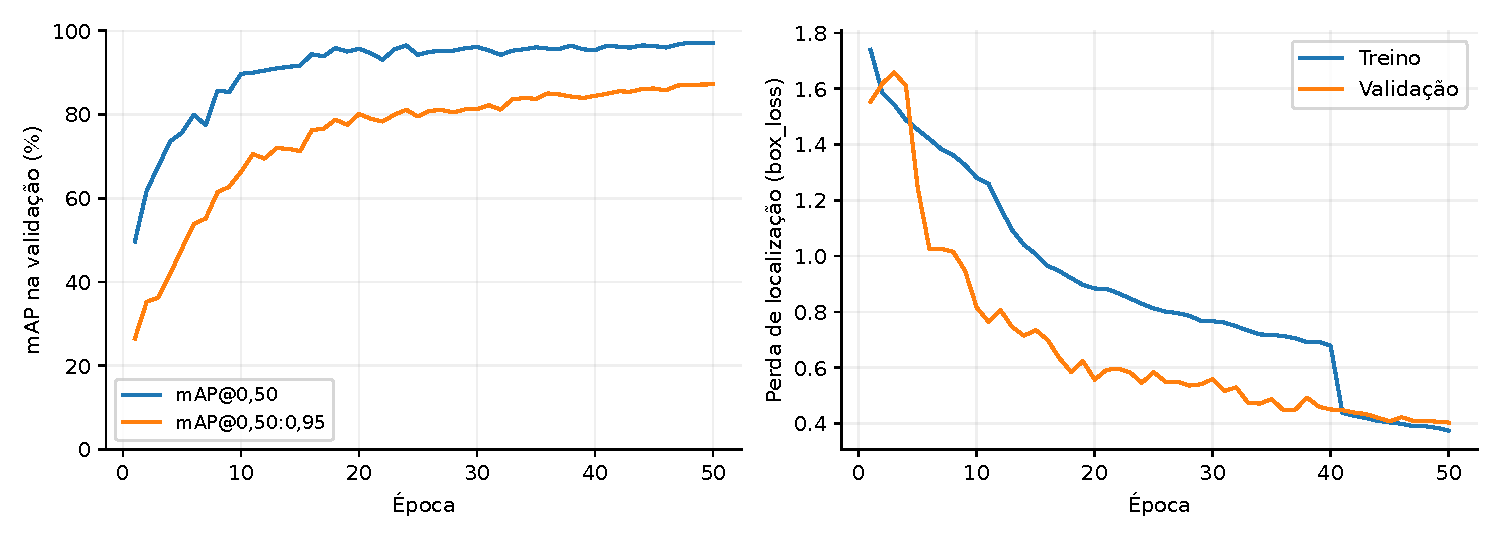
\includegraphics[width=\linewidth]{figuras/resultados_evolucao_treinamento.pdf}
\par\smallskip{\footnotesize Fonte: elaboração própria, com base nos registros do treinamento.\par}
\end{figure}



Na última época, a validação alcançou mAP@0,50 de 97,02\% e mAP@0,50:\allowbreak{}0,95 de 87,20\%. Este último foi o maior valor registrado nas 50 épocas. O checkpoint \texttt{best.pt}, selecionado com base nos resultados de validação, foi utilizado na avaliação do conjunto de teste. A diferença entre as duas medidas é esperada: a primeira admite uma correspondência espacial menos exigente, enquanto a segunda reúne avaliações com diferentes exigências de sobreposição entre as caixas. Conforme discutido por \textcite{padilla2021}, a interpretação do desempenho depende do critério de correspondência empregado. Por esse motivo, uma única medida de detecção não resume todos os aspectos da qualidade do modelo.


As curvas mostram avanço do aprendizado, mas não estabelecem uma duração ideal para o treinamento. As mudanças observadas ao final da execução devem ser interpretadas considerando também o encerramento do mosaico. Como as técnicas de aumento de dados não foram avaliadas isoladamente, o desempenho obtido corresponde ao conjunto de escolhas do experimento.

\vspace{\baselineskip}
\phantomsection
\addcontentsline{toc}{subsection}{4.2 Escolha do limiar de confiança para a contagem}
\noindent\textbf{4.2 Escolha do limiar de confiança para a contagem}\par
\nobreak\vspace{\baselineskip}\nobreak

Antes de contar os objetos no teste, foi necessário definir quais detecções seriam aceitas. Cada previsão recebe um valor de confiança; um limiar muito baixo permite incluir previsões incertas, enquanto um limiar muito alto pode descartar instrumentos que o modelo detectou com menor confiança. Essa escolha influencia diretamente tanto os objetos acrescentados indevidamente quanto os objetos que deixam de ser contados.

Foram avaliados 19 limiares, de 0,05 a 0,95, em intervalos de 0,05, exclusivamente no conjunto de validação. O critério principal foi minimizar a soma dos erros absolutos de contagem por categoria. Nesse cálculo, para cada imagem, comparou-se a quantidade prevista com a quantidade de referência em cada uma das sete categorias, somando as diferenças sem permitir que um excesso em uma categoria compensasse uma falta em outra.

O menor erro entre os valores examinados ocorreu no limiar 0,45, com soma de 71 erros absolutos por categoria e contagem correta em todas as categorias de 972 das 1.015 imagens de validação. A Figura~\ref{fig:res-limiar} mostra a variação do erro. O limiar 0,50 apresentou resultado próximo, com soma de 72, mas não superou o critério escolhido. Portanto, 0,45 foi adotado no teste; trata-se da melhor opção dentro da grade examinada, e não de uma demonstração de que seja o melhor valor possível em qualquer conjunto de imagens.

\begin{figure}[htbp]
\centering
\caption{Erro de contagem por categoria em função do limiar de confiança na validação}
\label{fig:res-limiar}
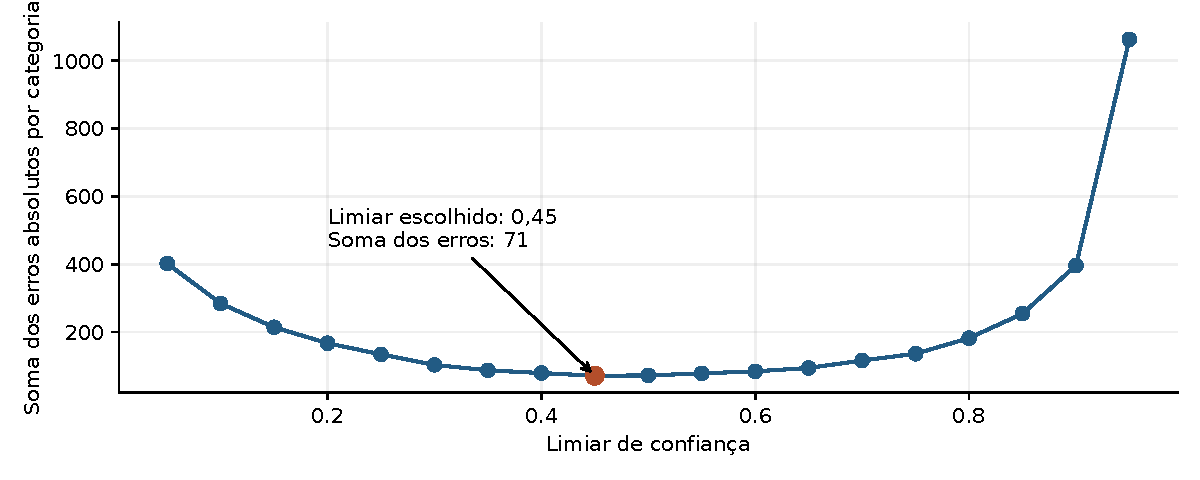
\includegraphics[width=.95\linewidth]{figuras/resultados_calibracao.pdf}
\par\smallskip{\footnotesize Fonte: elaboração própria, com base na calibração no conjunto de validação.\par}
\end{figure}

A escolha anterior ao teste preserva a finalidade desse conjunto: avaliar uma configuração já definida. Ajustar repetidamente o limiar a partir dos erros de teste reduziria a independência dessa avaliação. A revisão visual posterior foi empregada para compreender as falhas, sem modificar o limiar nem recalcular os resultados apresentados neste capítulo.

\vspace{\baselineskip}
\phantomsection
\addcontentsline{toc}{subsection}{4.3 Desempenho na detecção dos instrumentos}
\noindent\textbf{4.3 Desempenho na detecção dos instrumentos}\par
\nobreak\vspace{\baselineskip}\nobreak

Na avaliação padrão de detecção no teste, o modelo alcançou mAP@0,50 de 98,06\% e mAP@0,50:\allowbreak{}0,95 de 86,73\%. O resultado mais alto no primeiro critério mostra que a identificação com sobreposição mínima de 50\% foi mais favorável do que a avaliação que também exige delimitações mais próximas da referência. Assim, o modelo pode localizar a região do instrumento e ainda apresentar diferenças no tamanho ou na posição da caixa.

Para examinar o funcionamento da contagem, a Tabela~\ref{tab:res-deteccao} apresenta a precisão e a revocação calculadas com confiança de 0,45 e sobreposição mínima de 50\%. A precisão informa a proporção de detecções aceitas que corresponderam a objetos da categoria correta. A revocação informa a proporção dos objetos de referência que foi recuperada pelo modelo. Esses valores em um limiar fixo não devem ser confundidos com a precisão média, que considera a ordenação das previsões por confiança.

\begin{table}[htbp]
\centering
\caption{Detecção por categoria no ponto de operação adotado para a contagem}
\label{tab:res-deteccao}
\begin{minipage}{\linewidth}\small\singlespacing
\centering
\begin{tabular}{p{4.1cm}rrrr}
\hline
Categoria & Objetos & Acertos & Precisão (\%) & Revocação (\%) \\
\hline
Pinças & 509 & 497 & 97,26 & 97,64 \\
Tesouras & 451 & 442 & 99,33 & 98,00 \\
Afastadores & 81 & 78 & 91,76 & 96,30 \\
Porta-agulhas & 76 & 71 & 98,61 & 93,42 \\
Cabos de bisturi & 209 & 188 & 92,61 & 89,95 \\
Bicos de aspiração & 21 & 20 & 100,00 & 95,24 \\
Cúpulas & 30 & 30 & 96,77 & 100,00 \\
\hline
\end{tabular}
\par\smallskip\raggedright\footnotesize Fonte: elaboração própria.

Nota: objetos correspondem às anotações de referência utilizadas na avaliação; acertos representam detecções associadas à categoria correta com IoU $\geq 0{,}50$ e confiança $\geq 0{,}45$. Duas classificações incorretas da categoria porta-agulhas são examinadas na Seção~4.6.

\end{minipage}
\end{table}

Os cabos de bisturi apresentaram a menor revocação: 188 dos 209 objetos foram recuperados segundo o critério de correspondência. Também ocorreram 15 detecções incorretas nessa categoria. Nos afastadores, a precisão foi de 91,76\%, com sete detecções incorretas, enquanto três objetos não foram recuperados. Esses resultados indicam dificuldades diferentes: além de deixar de detectar objetos, o modelo pode gerar mais de uma previsão ou atribuir a categoria a uma região que não corresponde a um instrumento desejado.

As tesouras apresentaram precisão de 99,33\% e revocação de 98,00\%, com maior quantidade de objetos de referência do que os bicos de aspiração e as cúpulas. Para estas duas últimas categorias, os resultados favoráveis precisam ser interpretados à luz dos 21 e 30 objetos disponíveis no teste. A precisão de 100\% dos bicos de aspiração significa que não houve detecção incorreta dessa categoria neste conjunto; não significa ausência de falhas em novas situações. Da mesma forma, todas as cúpulas de referência foram recuperadas, mas houve uma detecção adicional incorreta.

\vspace{\baselineskip}
\phantomsection
\addcontentsline{toc}{subsection}{4.4 Contagem total e contagem por categoria}
\noindent\textbf{4.4 Contagem total e contagem por categoria}\par
\nobreak\vspace{\baselineskip}\nobreak

A contagem total coincidiu com a referência em 972 das 1.008 imagens, correspondendo a 96,43\%. Nas demais, houve subcontagem em 21 imagens e sobrecontagem em 15. O erro absoluto médio foi de 0,0536 objeto por imagem, calculado a partir da soma de 54 diferenças absolutas dividida pelas 1.008 imagens. Esse valor é uma média: não representa uma fração física de instrumento em cada fotografia e pode reunir muitos acertos com alguns erros maiores.

Ao exigir simultaneamente a quantidade correta em todas as sete categorias, o número de imagens com acerto diminuiu para 964, ou 95,63\%. Essa exigência corresponde à coincidência do vetor de contagens: além do total, cada posição da lista de quantidades por categoria deve estar correta. A diferença de oito imagens em relação ao acerto total mostra por que contar corretamente o conjunto não garante reconhecer corretamente sua composição. Um objeto atribuído à categoria errada pode preservar o total, mas altera duas posições dessa lista.

A soma dos erros absolutos por categoria foi de 76, equivalente à média de 0,0754 por imagem. Essa medida foi maior do que o erro da contagem total porque não permite compensações entre categorias. Considerando todas as imagens em conjunto, foram previstos 1.367 objetos, dez a menos do que os 1.377 da referência. Contudo, a diferença de dez no total agregado ocultaria erros locais de sentidos opostos. Para a conferência de uma fotografia, a comparação por imagem é mais informativa do que apenas somar todas as previsões do conjunto.



\begin{table}[htbp]
\centering
\caption{Erro absoluto médio da contagem por categoria no conjunto de teste}
\label{tab:res-mae-categorias}

\begin{minipage}{0.98\linewidth}
\singlespacing
\small
\centering

\begin{tabular}{lrrrr}
\hline
Categoria & Imagens positivas & Objetos & MAE geral & MAE positivo \\
\hline
Pinças             & 491 & 509 & 0,0218 & 0,0305 \\
Tesouras           & 340 & 451 & 0,0119 & 0,0294 \\
Afastadores        & 25  & 81  & 0,0079 & 0,3200 \\
Porta-agulhas      & 75  & 76  & 0,0060 & 0,0800 \\
Cabos de bisturi   & 191 & 209 & 0,0258 & 0,1309 \\
Bicos de aspiração & 20  & 21  & 0,0010 & 0,0500 \\
Cúpulas            & 30  & 30  & 0,0010 & 0,0000 \\
\hline
\end{tabular}

\par
\vspace{0.35em}
\raggedright
\footnotesize

Fonte: elaboração própria, a partir dos registros de avaliação do modelo (2026).

\par\vspace{0.25em}

\textit{Nota:} imagens positivas representam fotografias com pelo menos um objeto de referência da categoria. O MAE geral foi calculado sobre as 1.008 imagens de teste, incluindo aquelas sem objetos da categoria. O MAE positivo considera somente as imagens positivas da respectiva categoria. Ambos estão expressos em objetos por imagem.

\end{minipage}
\end{table}



Os cabos de bisturi apresentaram o maior MAE geral (0,0258), seguidos pelas pinças (0,0218). Entretanto, quando o cálculo considera somente as imagens positivas de cada categoria, destacam-se os afastadores, com MAE de 0,3200 em 25 imagens, e os cabos de bisturi, com 0,1309 em 191 imagens. Essa diferença evidencia como a baixa frequência de uma categoria pode reduzir seu erro médio quando todas as imagens do teste são consideradas. No caso das cúpulas, o MAE positivo foi nulo, enquanto o MAE geral foi de 0,0010, pois ocorreu uma previsão indevida em uma imagem sem objetos dessa categoria. Portanto, os dois indicadores são complementares: o MAE positivo caracteriza os erros de contagem nas imagens que contêm a categoria, enquanto o MAE geral também considera previsões indevidas em imagens nas quais ela está ausente. A quantidade desigual de imagens positivas deve ser considerada na comparação entre as categorias.


Além disso, a contagem correta não assegura uma delimitação correta. Uma previsão pode produzir o número esperado de objetos, mas apresentar uma caixa com sobreposição insuficiente em relação à referência. A avaliação conjunta das contagens e das detecções evita tratar esses casos como equivalentes a uma identificação inteiramente correta.

\vspace{\baselineskip}
\phantomsection
\addcontentsline{toc}{subsection}{4.5 Origem das imagens e quantidade de objetos na cena}
\noindent\textbf{4.5 Origem das imagens e quantidade de objetos na cena}\par
\nobreak\vspace{\baselineskip}\nobreak

A Tabela~\ref{tab:res-origem} separa os resultados pela origem das imagens. O acerto da contagem total foi de 98,39\% nas fotografias do HU-UEL e de 93,99\% nas imagens da internet. A coincidência das quantidades em todas as categorias também foi maior no subconjunto hospitalar.

\begin{table}[htbp]
\centering
\caption{Resultados de contagem por origem das imagens de teste}
\label{tab:res-origem}
\begin{minipage}{\linewidth}\small\singlespacing\centering
\begin{tabular}{p{2.3cm}rrrrr}
\hline
Origem & Imagens & Objetos & Total correto & Vetor correto & MAE total \\
\hline
HU-UEL & 559 & 647 & 98,39\% & 98,21\% & 0,0197 \\
Internet & 449 & 730 & 93,99\% & 92,43\% & 0,0958 \\
Conjunto & 1.008 & 1.377 & 96,43\% & 95,63\% & 0,0536 \\
\hline
\end{tabular}
\par\smallskip\raggedright\footnotesize Fonte: elaboração própria. Total correto e vetor correto representam proporções de imagens. MAE total: erro absoluto médio da quantidade total por imagem.
\end{minipage}
\end{table}

Essa diferença não demonstra que a origem hospitalar, isoladamente, tenha causado o melhor desempenho. Os subconjuntos diferem na composição de categorias, no número de objetos, no enquadramento e nas condições de captura. As fotografias hospitalares também podem compartilhar características visuais das sessões de aquisição presentes na base. Portanto, o resultado descreve o conjunto reservado para teste, sem equivaler a uma avaliação prospectiva em novos dias, ambientes ou rotinas de trabalho.

Há ainda uma restrição de cobertura: o subconjunto de teste do HU-UEL não contém cabos de bisturi anotados. Consequentemente, os resultados dessa categoria são provenientes das imagens da internet e não demonstram seu desempenho em fotografias hospitalares. Para porta-agulhas, bicos de aspiração e cúpulas do HU-UEL, foram avaliados, respectivamente, 18, 15 e 28 objetos, todos recuperados sem previsões adicionais dessas categorias nesse subconjunto. Embora favoráveis, essas observações abrangem amostras pequenas e condições limitadas de aquisição.

A quantidade de objetos na cena revela outra diferença importante. Das 1.008 imagens de teste, 845, ou 83,83\%, contêm apenas um objeto. Nesse grupo, a contagem total foi correta em 839 imagens, correspondendo a 99,29\%. Nas cenas com dois ou três objetos, o acerto foi de 84,31\%; nas cenas com quatro ou mais, foi de 78,43\%, como mostra a Figura~\ref{fig:res-cenas}.

\begin{figure}[htbp]
\centering
\caption{Acerto da contagem total conforme a quantidade de objetos de referência na cena}
\label{fig:res-cenas}
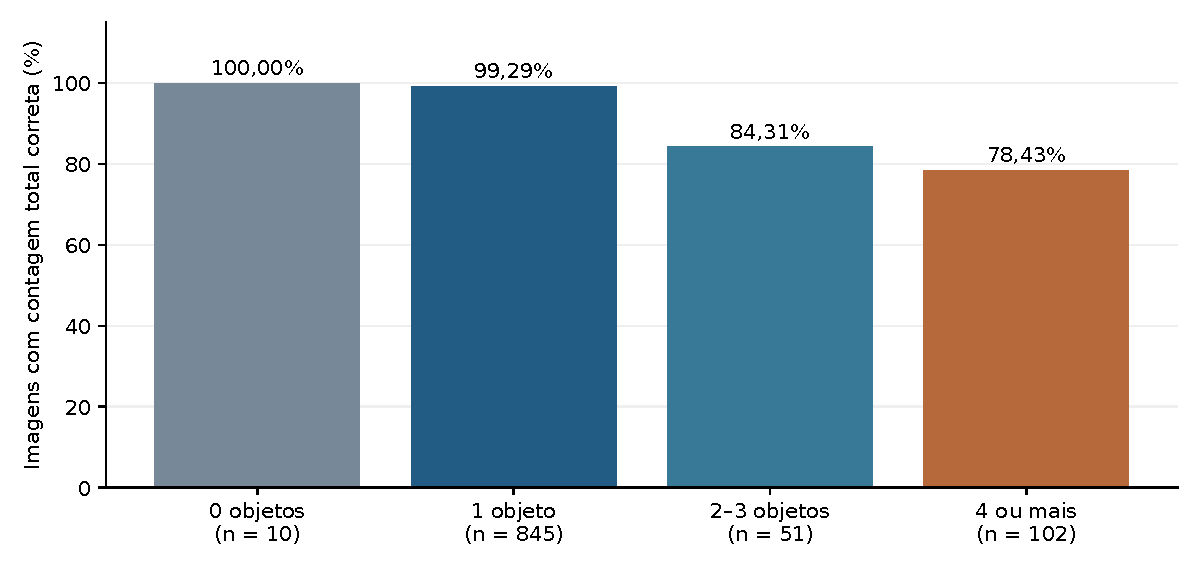
\includegraphics[width=.96\linewidth]{figuras/resultados_contagem_cenas.pdf}
\par\smallskip{\footnotesize Fonte: elaboração própria. O valor de $n$ indica a quantidade de imagens em cada grupo.\par}
\end{figure}

O erro absoluto médio também aumentou entre esses grupos: foi de 0,0107 nas imagens com um objeto, 0,1765 nas imagens com dois ou três e 0,3529 nas imagens com quatro ou mais. Esses números mostram uma associação entre cenas com mais objetos e maior dificuldade no conjunto avaliado. Como a composição das categorias e as condições das fotografias também variam, não é possível atribuir toda a diferença apenas ao número de instrumentos.

O grupo com quatro ou mais objetos reúne 102 imagens, das quais 100 possuem quatro objetos, uma possui cinco e uma possui dez. Assim, ele representa principalmente cenas com quatro instrumentos, e não bandejas completas com grande concentração de itens. As dez imagens sem objetos apresentaram contagem zero corretamente. Esse resultado é útil para verificar bandejas vazias, mas não demonstra que o modelo rejeitaria qualquer objeto estranho ou instrumento fora das categorias de interesse.

\vspace{\baselineskip}
\phantomsection
\addcontentsline{toc}{subsection}{4.6 Análise visual dos acertos e das falhas}
\noindent\textbf{4.6 Análise visual dos acertos e das falhas}\par
\nobreak\vspace{\baselineskip}\nobreak

Para compreender os resultados numéricos, foram examinadas visualmente 62 imagens: 30 selecionadas entre os maiores erros de contagem por categoria, duas com contagem correta e falha de correspondência espacial, 20 casos de acerto sorteados e dez imagens sem objetos. Essa seleção reúne situações úteis para análise, mas não constitui uma amostra aleatória de todo o teste. Portanto, a frequência de uma dificuldade nessa revisão não pode ser generalizada para todas as imagens.

Nos exemplos de acerto, as caixas delimitaram os instrumentos e receberam as categorias esperadas, inclusive em fotografias do HU-UEL. Nas falhas, foram observadas situações com instrumentos próximos ou sobrepostos, objetos visualmente semelhantes e regiões de baixo contraste. Essas observações ajudam a formular explicações para os erros, mas não isolam experimentalmente a contribuição de cada fator.

A Figura~\ref{fig:res-exemplos} apresenta dois casos. Na imagem dos afastadores Farabeuf, quatro objetos de referência resultaram em sete previsões. A proximidade e a sobreposição dos instrumentos dificultam distinguir suas partes e associá-las a um único objeto. No segundo exemplo, havia um cabo de bisturi de interesse e cinco lâminas; o modelo contou cinco objetos como cabos, incluindo quatro lâminas indevidamente. Esse caso mostra que uma categoria pode receber previsões de objetos com partes visualmente semelhantes, ainda que esses objetos não devam participar da contagem.

\begin{figure}[H]
\centering
\caption{Exemplos de sobrecontagem em afastadores e de confusão entre cabo de bisturi e lâminas}
\label{fig:res-exemplos}

\begin{minipage}[t]{0.49\linewidth}
\centering
{\small (a) Farabeuf: referência\par}
\vspace{0.2em}
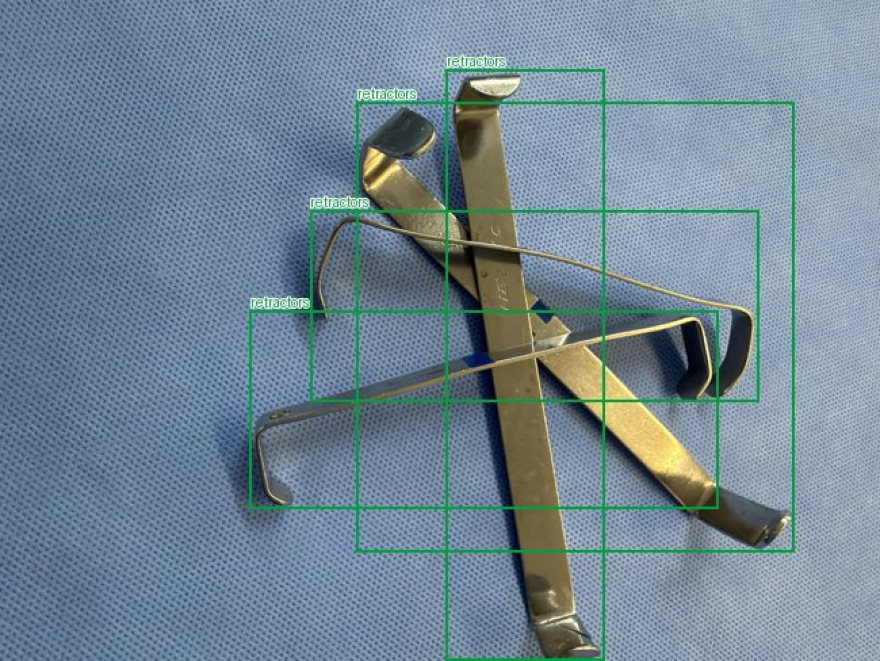
\includegraphics[width=\linewidth]{figuras/fig10_a_farabeuf_referencia.png}
\end{minipage}\hfill
\begin{minipage}[t]{0.49\linewidth}
\centering
{\small (b) Farabeuf: predição\par}
\vspace{0.2em}
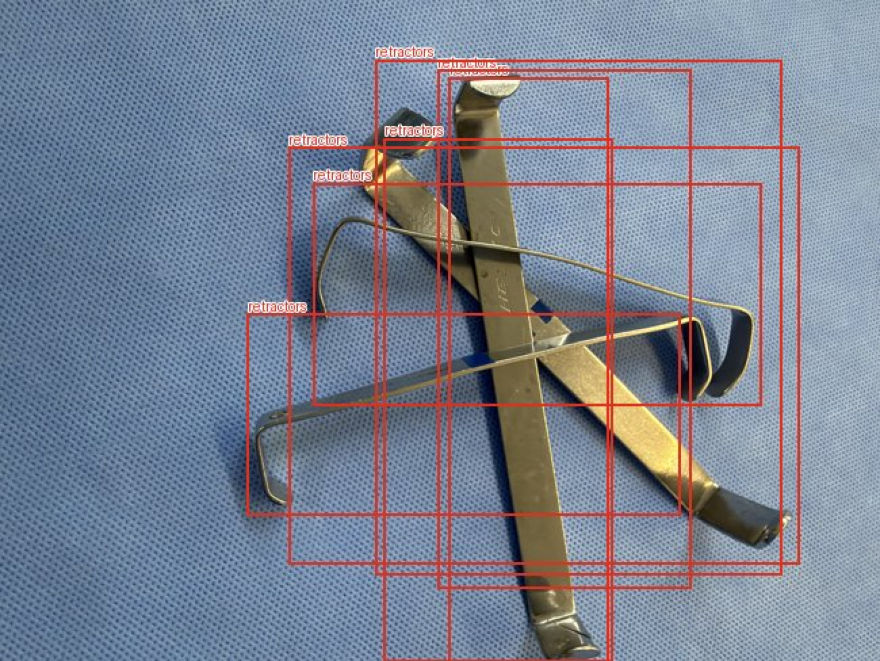
\includegraphics[width=\linewidth]{figuras/fig10_b_farabeuf_predicao.png}
\end{minipage}

\vspace{0.35cm}

\begin{minipage}[t]{0.49\linewidth}
\centering
{\small (c) Cabo e lâminas: referência\par}
\vspace{0.2em}
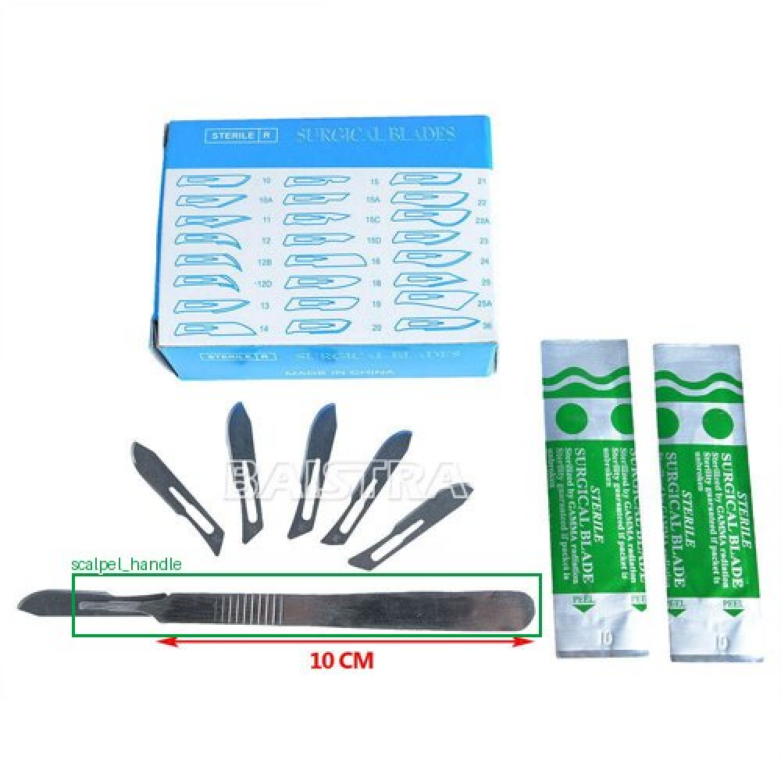
\includegraphics[width=\linewidth]{figuras/fig10_c_cabo_referencia.png}
\end{minipage}\hfill
\begin{minipage}[t]{0.49\linewidth}
\centering
{\small (d) Cabo e lâminas: predição\par}
\vspace{0.2em}
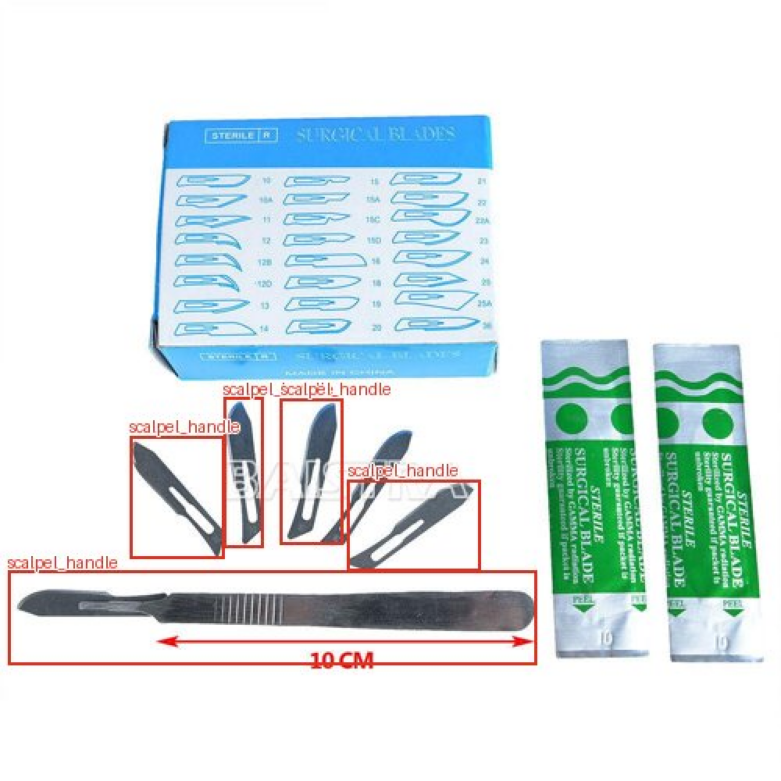
\includegraphics[width=\linewidth]{figuras/fig10_d_cabo_predicao.png}
\end{minipage}

\par\smallskip
{\footnotesize\raggedright
Fonte: elaboração própria, a partir das imagens do conjunto de teste e das saídas do modelo. Em (a) e (c), as caixas de referência aparecem em verde; em (b) e (d), as previsões aparecem em vermelho. Os identificadores em inglês correspondem às categorias utilizadas no processamento.\par}
\end{figure}

Também ocorreram omissões em fotografias com vários cabos de bisturi. Em um caso com cinco cabos lado a lado, foram detectados somente os dois externos. Em outro, com dez objetos de referência, foram previstos três. Esses exemplos ajudam a explicar por que a diferença entre o total previsto e o total de referência pode ser elevada em algumas imagens, apesar do erro médio reduzido no conjunto completo.


A revisão visual identificou ainda duas classificações incorretas nas anotações de referência: duas imagens de pinça Kelly reta haviam sido classificadas como porta-agulhas. Em ambos os casos, o modelo produziu uma previsão da categoria pinças, compatível com a identificação visual confirmada pela enfermeira colaboradora. Os resultados apresentados foram preservados conforme as anotações utilizadas na avaliação. Como análise de sensibilidade, considerando a correção dessas duas referências e mantendo as detecções e os 71 acertos originais da categoria porta-agulhas, sua revocação passaria de 93,42\% (71/76) para aproximadamente 95,95\% (71/74). Esse cálculo não constitui uma reavaliação completa das métricas, mas demonstra que parte do erro registrado decorre da referência utilizada, e não necessariamente de uma falha de identificação do modelo.

\vspace{\baselineskip}
\phantomsection
\addcontentsline{toc}{subsection}{4.7 Tempo de processamento e alcance dos resultados}
\noindent\textbf{4.7 Tempo de processamento e alcance dos resultados}\par
\nobreak\vspace{\baselineskip}\nobreak

O tempo de processamento foi medido em 50 imagens de teste, após três chamadas de aquecimento, com uma imagem por chamada e sincronização do processamento no dispositivo. A medição da chamada completa incluiu a leitura da imagem, o pré-processamento, a inferência e o pós-processamento. A média foi de 29,24 ms por imagem e a mediana de 24,22 ms. O percentil 95 foi de 48,81 ms, indicando que aproximadamente 95\% dos tempos medidos ficaram abaixo desse valor. O maior tempo observado foi de 281,13 ms, evidenciando que a duração não foi constante.

Esses valores sugerem rapidez para processar fotografias nas condições avaliadas. Entretanto, não incluem o tempo necessário para organizar os instrumentos, capturar a fotografia, transferi-la e conferir o resultado em uma aplicação completa. Também não equivalem a uma taxa de quadros validada em vídeo contínuo. O ganho de tempo na rotina hospitalar dependeria dessas etapas e exigiria uma avaliação própria do fluxo de trabalho.

A literatura oferece exemplos de detecção de instrumentos em condições distintas. \textcite{deol2024} avaliaram uma abordagem baseada em YOLOv9 com imagens contendo combinações de instrumentos, inclusive sobreposição e cenas com até 34 objetos. Esse tipo de cenário evidencia a importância de avaliar conjuntos mais densos. Contudo, diferenças no número de categorias, nas imagens, nas divisões dos dados e no protocolo impedem interpretar os valores de desempenho dos dois estudos como uma comparação direta de superioridade entre modelos.

A separação de imagens relacionadas entre treino, validação e teste também interfere na confiabilidade da avaliação. \textcite{kapoor2023} discutem como o vazamento de informação pode produzir estimativas excessivamente favoráveis em pesquisas com aprendizado de máquina. Nesta pesquisa, foram empregados agrupamentos e verificações de similaridade para reduzir esse risco. Esses procedimentos, porém, não demonstram independência completa entre todas as sessões de aquisição nem eliminam semelhanças que possam ter permanecido entre fotografias. Uma avaliação posterior com novas sessões de captura constitui uma forma importante de examinar essa limitação.

O experimento avaliou uma única configuração do YOLO26n, de modo que seus resultados não estabelecem superioridade em relação a outras variantes ou modelos. Além disso, uma operação do dispositivo MPS não dispunha de implementação determinística, o que limita a reprodução numérica exata mesmo com a semente fixada.

Os resultados sustentam uma viabilidade técnica inicial da detecção e da contagem por categorias gerais nas condições examinadas, especialmente em imagens com um instrumento e nas fotografias hospitalares representadas no teste. Essa conclusão é mais restrita do que afirmar que o sistema está pronto para conferir uma caixa cirúrgica completa. A redução do acerto nas cenas com vários objetos, a cobertura desigual das categorias e as falhas observadas em instrumentos próximos mostram a necessidade de ampliar a avaliação antes de propor seu uso como apoio à rotina. Assim, a principal contribuição desta etapa é demonstrar o potencial da abordagem e identificar, com dados de detecção e contagem, as condições que ainda exigem melhoria.

\endgroup

% Substitui os exemplos de referências do template.
\begingroup
\singlespacing
\setlength{\bibitemsep}{\baselineskip}
\raggedright
\setlength{\parindent}{0pt}
\phantomsection
\addcontentsline{toc}{section}{REFERÊNCIAS}
{\centering\bfseries REFERÊNCIAS\par}
\vspace{\baselineskip}
\printbibliography[heading=none]

\endgroup

%\include{20_referências2}
\include{21_glossario}
\include{22_apêndice}
\include{23_anexo}
\include{24_índice}

\end{document}